\documentclass[12pt]{report}
\usepackage[utf8]{inputenc}
\usepackage{graphicx}
\usepackage{xcolor}
\usepackage{soul}
\usepackage[colorlinks]{hyperref}
\usepackage{acronym}
\usepackage[backend=biber]{biblatex}
\usepackage{amsmath}
\usepackage{siunitx}
\usepackage[colorinlistoftodos]{todonotes}
\usepackage{tabularx}
\usepackage[toc,page]{appendix}

\setlength{\marginparwidth}{2cm}
\graphicspath{ {images/} }
\addbibresource{./references.bib}

% Equation formatting units
% https://tex.stackexchange.com/a/166610
\makeatletter
%%% redefine \eqref to be like the original
\renewcommand{\eqref}[1]{\textup{\eqreftagform@{\ref{#1}}}}
\let\eqreftagform@\tagform@
%%% redefine \tagform@
\def\tagform@#1{%
  \maketag@@@{%
    \if@unit(\thiseq@unit)\quad\fi\global\@unitfalse
    (\ignorespaces#1\unskip\@@italiccorr)%
  }%
}
\newif\if@unit
\def\equnit#1{%
  \gdef\thiseq@unit{#1}%
  \global\@unittrue
}
\makeatother

\setcounter{tocdepth}{4}
\setcounter{secnumdepth}{4}



% ----------- Begin actual document --------------
\begin{document}

\title {
    {Evaluation and Improvement of Photovoltaic Power Systems}\\
    {\large The University of Texas at Austin}\\
    {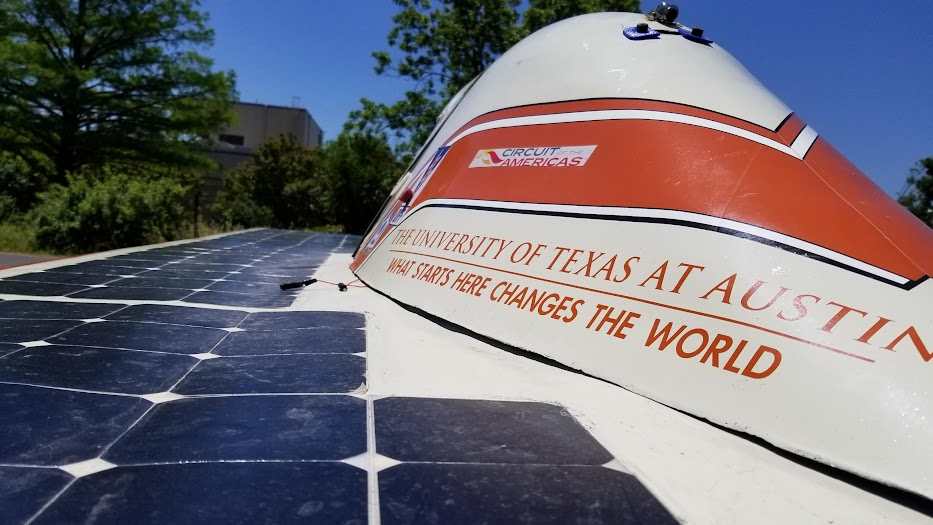
\includegraphics[width=\textwidth]{lonestar_cover.jpg}}
}
\author{Matthew Junkit Yu}
\date{20 December 2022}
\maketitle

{
    \hypersetup{linkcolor=black}
    \tableofcontents
    \listoffigures
    \listoftables
}

\chapter{Introduction}

In order to reach net zero emissions targets set by the \ac{UN} at the
2015 Paris Agreement~\cite{UN_Paris_agreement} before 2050, the \ac{IEA}
estimates that nearly 630 \ac{GW}~\cite{IEA_roadmap} of \ac{PV} energy
generation capacity need to be added annually by 2030. As of 2022, we observed
that at least 175 GW were installed in 2021~\cite{IEA_trends}~\cite{IEA_snapshot}, a 22\% year over year growth. With large policy and
geopolitical tailwinds behind major economies like the United States and Europe,
solar is expected to be one of the, if not the major driver of new energy
generation within the next two decades.

However, in order to achieve this target generation capacity in a sustainable
way, engineers and \ac{PV} designers need to maximize the electrical
efficiency of the overall power system, as opposed to just improving the solar
cell efficiency. According to the \ac{EIA}~\cite{EIA_capacity}, the capacity
factor of \ac{PV}s as an energy source in the United States reached a
monthly maximum of 33.4\% in June of 2022; \textit{capacity factor} is defined
by the \ac{EIA} as a measure of the generated output by the electric generator
versus the maximum possible output. It is clear that system inefficiencies in
\ac{PV} generation provide large constraints, and optimistically, equally
large opportunities, in allowing us to increase our pace towards reaching net
zero carbon emissions by 2050.

This thesis takes a holistic evaluation of the \ac{PV} power generation
system in a unique use case that necessitates maximizing the capacity factor:
solar powered vehicles. We evaluate the modeling, creation, and optimization of
a solar powered vehicle for the University of Texas at Austin's \ac{LHRs} team,
and attempt to identify and address inefficiencies and bottlenecks whose
improvements will help the larger \ac{PV} industry as a whole.

In particular, this thesis will focus on three important and active areas of
development within the \ac{PV} field: solar array modeling and prediction,
\todo{The second area of development may be more generalized then this.}
\hl{solar cell binning processes and heuristics},
and \ac{MPPT} algorithms.
In each of these areas, we look at the state of the art techniques, propose novel
ideas to improve our understanding of the system and its inefficiencies, and see
if we can translate it lateral applications like rooftop solar or industrial
\ac{PV}.\@ Note that in this thesis we refer to photovoltaics and solar without
distinction.

In the first major chapter, \textbf{Modeling Photovoltaics}, this thesis
discusses how can solar cells can be modeled at various abstraction layers, from
idealized cells at standard conditions using the 3-parameter model to
non-idealized cells that incorporate parasitic resistances using the 7-parameter
model. These solar cell models are then evaluated against a dataset of several
hundred solar cell \ac{I-V} and \ac{P-V} curves generated from our custom
testing setup to see how well the model fits real cells at different conditions.
We build upon these models to form larger units of \ac{PV}s, such as solar
modules and solar arrays, which may consist of strings of cells in series with
bypass diodes across them, among other configurations. Some important topics
that are explored using these multi-cell models include \ac{PV} mismatch and
bypass activation. Insights from these topics lead to heuristics that are
proposed in the next chapter, \textbf{Optimizing Photovoltaics}.

The second major chapter, \textbf{Optimizing Photovoltaics}, takes the
aforementioned models and dataset created to propose a process to bin, match,
and combine solar cells and modules, with the end goal of maximizing the
performance of the solar array that will be attached to the solar vehicle. In
this chapter, we propose design criteria, heuristics, and methodologies to
generate designs for the solar vehicle that fit the unique constraints of the
application, which center around the dynamism of the system as it moves in
transit across the real world.

In the third and final major chapter, \textbf{Optimizing Photovoltaic
Systems}, this thesis investigates the operation of the \ac{PV}
system in the context of the solar vehicle. We observe the energy conversion
process from incident light on the solar array to electricity captured by the
\ac{BPS} and present a \ac{PV} system simulator and a suite of \ac{MPPT}
algorithms to minimize energy losses from the aforementioned conversion process.
We demonstrate custom hardware developed by the \ac{LHRs} team and evaluate in
real world settings a select set of \ac{MPPT} algorithms. We compare these
results with existing research and our digital twin model of the solar vehicle,
and finally discuss conclusions from the three chapters that can be translatable
to the wider \ac{PV} industry.

Along with these three major chapter, we also provide a large set of appendices
corresponding to the development of the main body of work in this thesis. Among
them include manufacturing procedures for testing, assembling, and laminating
solar cells into solar modules, schematics and accompanying documentation for
hardware that was used for characterizing and validating parts of the thesis,
software diagrams with relevant open source software repositories developed by
our team, and extra insights into the design of the \ac{LHRs}' photovoltaic
array that are not directly applicable to the major chapters, such as thermal
models performed of the vehicle topshell that influenced our simulation models,
among others.

\chapter{Modeling Photovoltaics}\label{chapter:modeling_pvs}

In this chapter, \textbf{Modeling Photovoltaics}, we systematically review the
various types of abstractions in photovoltaics, starting from solar cells and
ending with solar arrays.

We start by observing how solar cell models themselves can have differing
granularities in their composition and how they address an array of internal
qualities and external environs that influence real world performance. We also
propose modifications that may improve their accuracy and precision, and
consider tradeoffs that may occur in nonnominal conditions. We then evaluate
these models against a dataset of solar cells characterized for use on the
\ac{LHRs} vehicle, and then use the `best' set of models to predict solar cell
behavior in larger contexts.

These larger contexts start with the formation of solar modules that can take
multiple shapes and sizes. We attempt to use the base set of models to
understand how different configurations of solar modules may be affected by
photovoltaic mismatch, a phenomenon caused by nonuniform cells in series or in
parallel, either through manufacturing defects or lighting and thermal
gradients across the module. We also add a bypass diode component in
antiparallel to the solar module models in order to evaluate their turn-on
conditions and mismatch mitigation effects. From these solar module models, we
formulate a metric to measure mismatch, and propose suggestions on module size
and bypass diode selection that can minimize mismatch. These suggestions will
become heuristics and algorithms for optimizing module design later on in
\autoref{chapter:optimizing_pvs}.

Finally, we take these solar module models and combine them together to form a
cohesive solar array model. From this model, we observe how the individual
module effects can generate a global \ac{I-V} curve with local and global
maxima, and discuss how this curve impacts how the larger photovoltaic system
interacts with solar arrays.

\newpage
\section{Three Parameter Solar Cell Model}\label{sec:three_parameter_solar_cell_model}

\subsection{Model Introduction}\label{subsec:three_param_model_introduction}

\begin{figure}[h]
    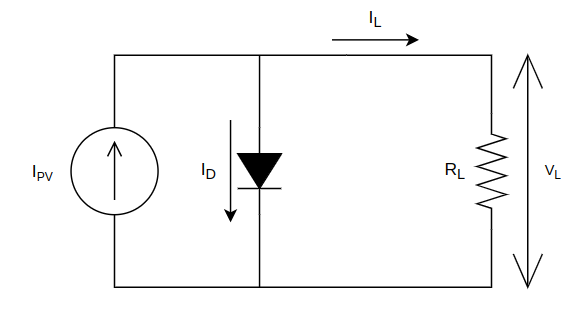
\includegraphics[width=\textwidth]{solar_cell_three_parameter_model.png}
    \caption{Three Parameter, or Single Diode Model of a Solar Cell}
    \label{fig:single_diode_model}
\end{figure}

The most basic model of a solar cell is the three parameter model, or single
diode model, shown in \autoref{fig:single_diode_model}. It consists of a
constant current source and a diode. The constant current source produces a
\ac{IPV} caused by photons of sufficient energy being absorbed into the surface
of the solar cell and exciting charge carriers (generally in the form of
electrons) to enter the circuit. The diode represents the various recombination
processes that consume the generated current in the form of \ac{ID}.

In this model, the three parameters consist of the following:

\begin{itemize}
    \item \acf{IPV},
    \item \acf{I0},
    \item and an \acf{N}.
\end{itemize}

The latter two are contained within the dark current term, and generally
influence the shape of the predicted \ac{I-V} curve, particularly around the
knee-bend.

This model is juxtaposed from the five parameter model in that it does not
incorporate cell losses in the form of \ac{RS} and \ac{RSH}. It is assumed that
in this model, the series resistance is zero (short circuit) and the shunt
resistance is infinite (open circuit). Therefore, the five parameter model may
also be called the complete single diode model.

We observe from \autoref{fig:single_diode_model} that the \ac{IL} can be
represented as a function of the photocurrent and the dark current, shown in
\autoref{eq:cell_output_current_1}.

\begin{equation}
    I_L = I_{PV} - I_D
    \equnit{\si{\ampere}}
    \label{eq:cell_output_current_1}
\end{equation}

In the following subsections, we break down each component into its constituent
parts.


\subsection{Photocurrent}\label{subsec:three_param_photocurrent}

\begin{equation}
    I_{PV} = qA\int_{}{}b_s(E)QE(E)dE
    \equnit{\si{\ampere}}
    \label{eq:cell_photocurrent_1}
\end{equation}

On a fundamental level, we can define the \acf{IPV} as a function of the photons
incident upon the surface of the solar cell and the solar cell's spectral
response. This is demonstrated in \autoref{eq:cell_photocurrent_1}. A bulleted,
simplistic explanation of this equation is presented as follows:

\begin{itemize}
    \item Incident light hits the solar cell over a given spectrum of energy
    levels (denoted either in $eV$ or in $nm$) (see
    \autoref{fig:maxeon_gen_iii_cell_spectral_response}).
    \item Incident light at each discrete energy level has an \ac{BS}, otherwise
    known as intensity.
    \item The solar cell has a given \ac{QE} at each energy level that is the
    probability that an incident photon of \ac{E} delivers one electron to the
    external circuit.
    \item Integrating the product of the photon flux density \ac{BS} and quantum
    efficiency \ac{QE} (then multiplied by the \ac{Q} and the cell \ac{A})
    provides the photocurrent (\ac{IPV}).
\end{itemize}

\begin{figure}[h]
    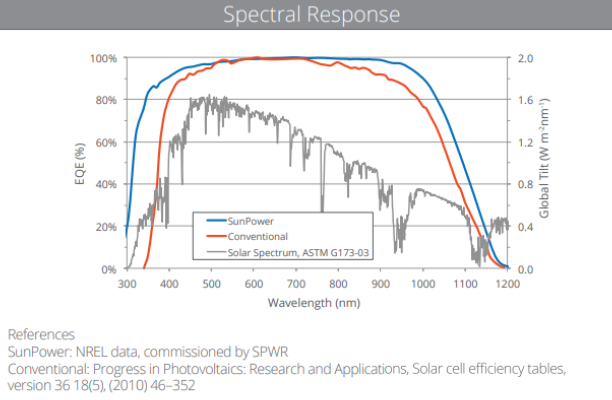
\includegraphics[width=\textwidth]{maxeon_gen_iii_cell_spectral_response.png}
    \caption{Maxeon Gen III Cell Spectral Response}
    \label{fig:maxeon_gen_iii_cell_spectral_response}
\end{figure}

Solar cell manufacturers may provide a spectral response chart showing the
quantum efficiency over the useful solar spectrum (as seen in
\autoref{fig:maxeon_gen_iii_cell_spectral_response}), but will generally just
provide the \ac{ISC} at \ac{STC} ($1000$ $Wm^{-2}$, $AM$ $1.5G$, $25$ $C$).

As it turns out, the photocurrent can generally be approximated as the short
circuit current. We'll discuss in \autoref{subsec:five_param_series_resistance}
that Cubas et al.~\cite{cubas_et_al}\cite{cubas_et_al_2} defines the
photocurrent as a ratio of the series and shunt resistance in addition to the
short circuit current. However, in most cases, the empirical value of \acl{ISC}
will not differ from \autoref{eq:cell_photocurrent_2}.

\begin{equation}
    I_{PV} = I_{SC}
    \equnit{\si{\ampere}}
    \label{eq:cell_photocurrent_2}
\end{equation}


\subsection{Dark Current}\label{subsec:three_param_dark_current}

The \acf{ID} comprises of the interesting and critical parameters of the three
parameter model; shown in \autoref{eq:cell_dark_current_1}, it consists of the
term \ac{I0} and an exponential. The exponential is a function of three key
variables: the \acf{TC}, \acf{VL}, and \acf{N}.

\begin{equation}
    I_D = I_0[\exp(\frac{V}{V_T}) - 1]
    \equnit{\si{\ampere}}
    \label{eq:cell_dark_current_1}
\end{equation}

This ideality factor is typically between $1$ and $2$, and represents the
proportional influence of carriers inbseveral recombination processes for a
given cell composition and structure. Some ideality factor values are presented
in \autoref{table:ideality_factors}, sourced from PVEducation's Ideality Factor
page~\cite{pveducation_ideality_factor}. We note that the ideality factor may be
outside the typical range of $[1, 2]$, as discussed by Jain et
Kapoor~\cite{jain_et_kapoor} and R.N. Hall~\cite{hall}, the latter of which
notes that auger recombination dominated dark currents may generate a \ac{N} of
$2/3$.

The term \ac{VT} (\autoref{eq:cell_thermal_voltage}) which encapsulates the cell
temperature dependency describes the voltage across the P-N junction of the
diode in the model: at \ac{STC} this is typically $26$ $mV$. We remind the
reader that the remaining terms in this equation are the \acf{KB} and \acf{Q}.

\begin{equation}
    V_T = \frac{n k_B T_C}{q}
    \equnit{\si{\volt}}
    \label{eq:cell_thermal_voltage}
\end{equation}

\begin{table}[h!]
    \begin{tabularx}{\textwidth}{
        | >{\raggedright\arraybackslash}X
        | >{\raggedright\arraybackslash}X
        | >{\raggedright\arraybackslash}X | }
        \hline
        Recombination Type & Ideality Factor & Description \\ \hline \hline
        SRH, band to band (low level injection) & 1 & Recombination limited by minority carrier. \\ \hline
        SRH, band to band (high level injection) & 2 & Recombination limited by both carrier types. \\ \hline
        Auger & 2/3 & Two majority and one minority carriers required for recombination. \\ \hline
        Depletion region (junction) & 2 & Two carriers limit recombination. \\ \hline
    \end{tabularx}
    \caption{Various Ideality Factors of \ac{N}}
    \label{table:ideality_factors}
\end{table}


\subsection{Dark Saturation Current}\label{subsec:three_param_dark_sat_current}

The \acf{I0} has two potential derivations. Generally, the three parameter
model, (see Baig et al.~\cite{baig_et_al}, MacAlpine et
Brandemuehl~\cite{macalpine_et_brandemuehl}, Rusirawan et
Farkas~\cite{rusirawan_et_farkas}, and others) define \ac{I0} as in
\autoref{eq:cell_dark_sat_current_1}; where the diode current is a function of
the cell temperature and the energy bandgap in relation to several reference
parameters at \ac{STC}.

\begin{equation}
    I_0 = I_{0,ref}{(\frac{T_C}{T_{C,ref}})}^3\exp(\frac{E_{G,ref}}{k_B T_{C,ref}} - \frac{E_G}{k_B T_C})
    \equnit{\si{\ampere}}
    \label{eq:cell_dark_sat_current_1}
\end{equation}

On the other hand, we can derive the \ac{I0} algebraically: given the short
\acf{ISC} and \ac{VOC}, we can set the cell at open circuit,
forming the derivation in \autoref{eq:cell_dark_sat_current_deriv} and the
result in \autoref{eq:cell_dark_sat_current_2}.

\begin{equation}
    \begin{split}
        I_L &= 0 \\
        & = I_{SC} - I_D \\
        & = I_{SC} - I_0[\exp(\frac{V_{OC}}{V_T}) - 1]
    \end{split}
    \equnit{\si{\ampere}}
    \label{eq:cell_dark_sat_current_deriv}
\end{equation}

\begin{equation}
    I_0 = I_{SC}[\exp(\frac{V_{OC}}{V_T}) - 1]^{-1}
    \equnit{\si{\ampere}}
    \label{eq:cell_dark_sat_current_2}
\end{equation}

The latter model is convenient since it does not require measuring \ac{I0REF},
\ac{EGREF}, nor \ac{EG}. As such, we will only evaluate the latter model in
\autoref{sec:evaluation_of_solar_cell_models}.


\subsection{Short Circuit Current}\label{subsec:three_param_short_circuit_current}

Finally, for the three parameter model, we derive the dependence of \acf{ISC}
and \acf{VOC} on \acf{G} and \acf{TC} before establishing the final derivation
of \autoref{eq:cell_output_current_1}.

Starting with the \acf{ISC}, it is known that there is a large positive
correlation with irradiance and a small positive correlation with temperature,
shown in \autoref{fig:cell_temperature_dependence} and
\autoref{fig:cell_irradiance_dependence}.

\begin{figure}[!htbp]
    \centering
    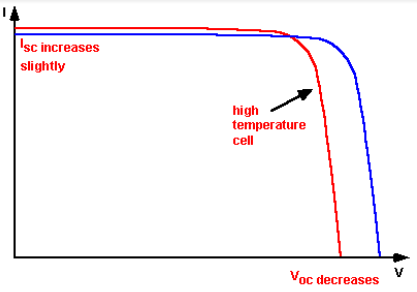
\includegraphics[width=0.7\linewidth]{cell_temperature_dependence.png}
    \caption{Solar Cell Temperature Dependence}
    \label{fig:cell_temperature_dependence}
\end{figure}

\begin{figure}[!htbp]
    \centering
    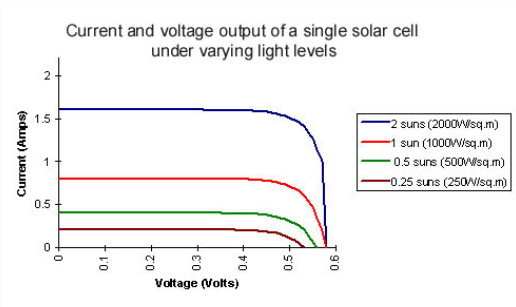
\includegraphics[width=0.9\linewidth]{cell_irradiance_dependence.png}
    \caption{Solar Cell Irradiance Dependence}
    \label{fig:cell_irradiance_dependence}
\end{figure}

The dependence of irradiance on $I_{SC}$ can be modeled as linearly proportional
to the light incident upon the solar cell over the reference irradiance. This
makes intuitive sense: given half the available light (assuming the distribution
of light across the spectrum is consistent), the solar cell will only be able to
capture half the maximum available power. Chegaar et al.~\cite{chegaar_et_al}
proposes this relationship as \autoref{eq:cell_short_circuit_current_1}, where
the short circuit current is a function of \ac{KE} and \acf{G} (the latter in
units of $Wm^{-2}$).

\begin{equation}
    I_{SC}(G) = K_E G
    \equnit{\si{\ampere}}
    \label{eq:cell_short_circuit_current_1}
\end{equation}

\autoref{eq:cell_short_circuit_current_1} can be easily reworked where the
constant \ac{KE} is now based on a \acf{ISCREF} and a \ac{GREF}. This forms
\autoref{eq:cell_short_circuit_current_2}, which is the same form used by Baig
et al.~\cite{baig_et_al}.

\begin{equation}
    I_{SC}(G) = I_{SC,ref}\frac{G}{G_{ref}}
    \equnit{\si{\ampere}}
    \label{eq:cell_short_circuit_current_2}
\end{equation}

Hishikawa et al.~\cite{hishikawa_et_al} proposes modeling the dependence of
temperature on \ac{ISC} using a \acf{ALPHA}
(\autoref{eq:thermal_coefficient_alpha}). \ac{ALPHA} is empirically determined
and varies given the material composition and structure of the solar cell; for
crystalline silicon solar cells, this is approximately 0.05\%/K, or 0.0005.
\autoref{eq:thermal_coefficient_alpha} can be rearranged to form
\autoref{eq:cell_short_circuit_current_3}. This is effectively equivalent to
Rusirawan et Farkas~\cite{rusirawan_et_farkas}, but is slightly different from
MacAlpine et Brandemuehl~\cite{macalpine_et_brandemuehl} and Baig et
al.~\cite{baig_et_al}, who take the constant term $1$ and replace it with a
another constant, \ac{ISCREF} (\autoref{eq:cell_short_circuit_current_4}).

\begin{equation}
    \alpha = \frac{1}{I_{SC,ref}}\frac{\Delta I_{SC}}{\Delta T_C} = \frac{1}{I_{SC,ref}}\frac{I_{SC,ref} - I_{SC}}{T_{C,ref} - T_C}
    \equnit{\si{unitless}}
    \label{eq:thermal_coefficient_alpha}
\end{equation}

\begin{equation}
    I_{SC}(T_C) = I_{SC,ref}[1 - \alpha(T_{C,ref} - T_C)]
    \equnit{\si{\ampere}}
    \label{eq:cell_short_circuit_current_3}
\end{equation}

% NOTE: Rusirawan et Farkas derivation to match short_circuit_current_3.
% \begin{equation}
%     \mu = \frac{I_{SC} - I_{SC,ref}}{T_C - T_{C,ref}} = -\alpha I_{SC,ref}
%     \equnit{\si{unitless}}
% \end{equation}
% \begin{equation}
%     I_{SC}(T_C) = I_{SC,ref}+\mu(T_{C,ref} - T_C), where
%     \equnit{\si{\ampere}}
%     \label{eq:cell_short_circuit_current_4}
% \end{equation}

\begin{equation}
    I_{SC}(T_C) = I_{SC,ref}[I_{SC,ref} - \alpha(T_{C,ref} - T_C)]
    \equnit{\si{\ampere}}
    \label{eq:cell_short_circuit_current_4}
\end{equation}

These two competing models of the short circuit current will also be explored
further in \autoref{sec:evaluation_of_solar_cell_models}. For the purposes of
this subsection, however, we will combine
\autoref{eq:cell_short_circuit_current_2} and
\autoref{eq:cell_short_circuit_current_3} to give us
\autoref{eq:cell_short_circuit_current_5}.

\begin{equation}
    I_{SC}(G, T_C) = I_{SC,ref}\frac{G}{G_{ref}}[1 - \alpha(T_{C,ref} - T_C)]
    \equnit{\si{\ampere}}
    \label{eq:cell_short_circuit_current_5}
\end{equation}


\subsection{Open Circuit Voltage}\label{subsec:three_param_open_circuit_voltage}

Likewise, the \acf{VOC} is also a function of temperature and
irradiance. It is known that \ac{VOC} has a medium positive
correlation with irradiance and a medium negative correlation with temperature
(\autoref{fig:cell_temperature_dependence} and
\autoref{fig:cell_irradiance_dependence}).

Returning to \autoref{eq:cell_dark_sat_current_2}, in which we defined the
\acf{I0} as a function of \ac{VOC}, we can invert the equation to retrieve the
\ac{VOC} parameter, shown in \autoref{eq:cell_open_circuit_voltage_1}.

\begin{equation}
    V_{OC} = V_T\ln(\frac{I_{SC}}{I_0} + 1)
    \equnit{\si{\volt}}
    \label{eq:cell_open_circuit_voltage_1}
\end{equation}

There are three points in this equation that can now be determined. We know from
\autoref{eq:cell_thermal_voltage} that the \acf{VT} is dependent on the
\acf{TC}. We can also plug in one of the proposed models for \ac{ISC}. However,
we cannot reuse \autoref{eq:cell_dark_sat_current_2} because
\autoref{eq:cell_open_circuit_voltage_1} was derived from it! Chegaar et
al.~\cite{chegaar_et_al} proposes an alternative form by simplifying the
logarithmic term to form \autoref{eq:cell_open_circuit_voltage_2}.

\begin{equation}
    V_{OC}(G, T_C) = V_{OC,ref} + V_T(T_C)\ln(\frac{G}{G_{ref}} + 1)
    \equnit{\si{\volt}}
    \label{eq:cell_open_circuit_voltage_2}
\end{equation}

This term fits well with the paper’s experimental data, but is not immediately
clear how it models the original term. It also does not properly model
temperature change. \autoref{eq:cell_open_circuit_voltage_3} is a modified
form that implements temperature dependence while retaining irradiance
dependence.

\begin{equation}
    \begin{split}
        V_{OC}(G, T_C) &= V_{OC,ref}[1 - \beta (T_{C,ref} - T_C)] \\
        & \quad+ \frac{nk_B(T_{C,ref} + T_C/\gamma)}{q}\ln(\frac{G}{G_{ref}})
    \end{split}
    \equnit{\si{\volt}}
    \label{eq:cell_open_circuit_voltage_3}
\end{equation}

\begin{equation}
    \beta = \frac{1}{V_{OC,ref}}\frac{\Delta V_{OC}}{\Delta T_C}
          = \frac{1}{V_{OC,ref}}\frac{V_{OC,ref} - V_{OC}}{T_{C,ref} - T_C}
    \equnit{\si{unitless}}
    \label{eq:thermal_coefficient_beta}
\end{equation}

\autoref{eq:cell_open_circuit_voltage_3} implements two changes: a \acf{BETA}
and a \acf{GAMMA}. \ac{BETA} is likewise (to \ac{ALPHA}) empirically determined;
for silicon it known to be -0.3\%/K, or -0.003. \ac{GAMMA} is an experimentally
determined curve fitting term, and may more appropriately model the exponential
decrease of \ac{VOC} at low light conditions. It has an expected operable range
of values between $[1, 100]$, where smaller values correlate to a wider range of
of \ac{VOC} movement at low light conditions. This parameter, however, is not
part of the three parameter cell model. Its efficacy will be explored further in
\autoref{sec:evaluation_of_solar_cell_models}.


\subsection{Model Summary}\label{subsec:three_param_model_summary}

To conclude this section, we will review the components that make up the three
parameter cell model, propose three items of further exploration, and propose a
complete model function that incorporates the topics discussed.

Firstly, the three parameter cell model is composed of a constant current source
and a power consuming diode, representing photogeneration and recombination
effects of the solar cell, respectively. These two components form three
parameters that is the namesake of this section, namely the photocurrent, dark
saturation current, and ideality factor.

Secondly, we explore the construction and interpretation of these three
components, and along the way, examine three areas that deviate from the
existing models that we would like to investigate:

\begin{itemize}
    \item an algebraic derivation of the \acf{I0},
    \item an alternative interpretation of the \acf{ISC} as
    a function of \acf{TC},
    \item and a new \acf{GAMMA} to improve \acf{VOC} modeling at low lighting
    conditions.
\end{itemize}

Finally, we present the complete model and its derivation, in
\autoref{eq:cell_output_current_2}. We observe that this complete model requires
four reference parameters (note that in this paragraph we refer to parameters as
in values that need to be determined and not larger terms used in the naming of
the model):

\begin{itemize}
    \item \acf{GREF}
    \item \acf{TCREF}
    \item \acf{VOCREF}
    \item \acf{ISCREF}
\end{itemize}

and four curve fitting parameters:

\begin{itemize}
    \item \acf{N}
    \item \acf{ALPHA}
    \item \acf{BETA}
    \item \acf{GAMMA}
\end{itemize}

For the cells tested in this project, \ac{ALPHA} and \ac{BETA} were provided
by the manufacturer, Maxeon, but \ac{N} and \ac{GAMMA} were not. Curve fitting
techniques, like simulated annealing, will have to be applied to determine these
two variables, and are explored in
\autoref{sec:evaluation_of_solar_cell_models}.


% TODO: This is equation is a freak of nature... Probably stop at second to last
% step and move most of the derivation to an appendix.
\todo{Reformat this equation}
\begin{equation}
    \begin{split}
        I_L(V_L, G, T_C) &= I_{PV}(G, T_C) - I_D(V_L, G, T_C) \\
        & = I_{SC}(G, T_C) - I_D(V_L, G, T_C) \\
        & = I_{SC}(G, T_C) - I_0[\exp(\frac{V_L}{V_T(T_C)}) - 1] \\
        & = I_{SC}(G, T_C) - I_{SC}(G, T_C)[\exp(\frac{V_{OC}(G, T_C)}{V_T(T_C)}) - 1]^{-1}[\exp(\frac{V_L}{V_T(T_C)}) - 1] \\
        & = I_{SC}(G, T_C) - I_{SC}(G, T_C)\frac{\exp(\frac{V_L}{V_T(T_C)}) - 1}{\exp(\frac{V_{OC}(G, T_C)}{V_T(T_C)}) - 1} \\
        & = I_{SC}(G, T_C) - I_{SC}(G, T_C)\frac{\exp(\frac{qV_L}{n k_B T_C}) - 1}{\exp(\frac{qV_{OC}(G, T_C)}{n k_B T_C}) - 1} \\
        & = I_{SC}(G, T_C)[1 - \frac{\exp(\frac{qV_L}{n k_B T_C}) - 1}{\exp(\frac{qV_{OC}(G, T_C)}{n k_B T_C}) - 1}] \\
        & = I_{SC,ref}\frac{G}{G_{ref}}[1 - \alpha[T_{C,ref} - T_C]][1 - \frac{\exp(\frac{qV_L}{n k_B T_C}) - 1}{\exp(\frac{qV_{OC}(G, T_C)}{n k_B T_C}) - 1}] \\
        & = I_{SC,ref}\frac{G}{G_{ref}}[1 - \alpha[T_{C,ref} - T_C]] \\
        & \quad* [1 + \frac{1 - \exp(\frac{qV_L}{n k_B T_C})}{1 - \exp(\frac{q[V_{OC,ref}[1 - \beta[T_{C,ref} - T_C]] + \frac{nk_B(T_{C,ref} + T_C/\gamma)}{q}\ln(\frac{G}{G_{ref}})]}{n k_B T_C})}] \\
    \end{split}
    \equnit{\si{\ampere}}
    \label{eq:cell_output_current_2}
\end{equation}

\todo[inline]{See \url{https://www.desmos.com/calculator/yp0rhmabkz} to play
around with the complete three parameter solar cell model. Add as a figure later
on compared to experimental data.}

\newpage
\section{Five Parameter Solar Cell Model}\label{sec:five_parameter_solar_cell_model}

\subsection{Model Introduction}\label{subsec:five_param_model_introduction}

\begin{figure}[h]
    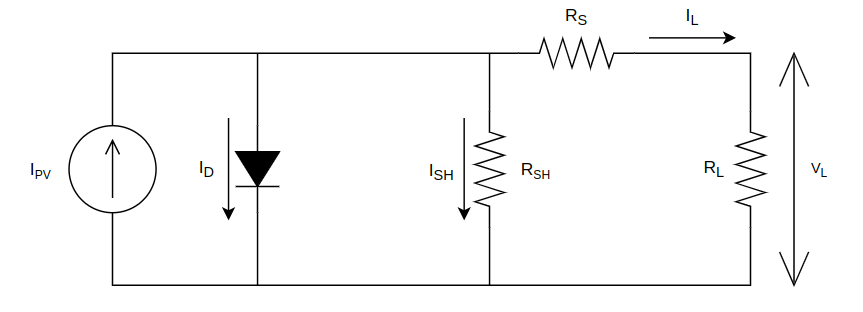
\includegraphics[width=\textwidth]{solar_cell_five_parameter_model.png}
    \caption{Five Parameter, or Full Single Diode Model of a Solar Cell}
    \label{fig:single_diode_model_with_resistances}
\end{figure}

The most common model for solar cells is the five parameter solar cell model,
shown in \autoref{fig:single_diode_model_with_resistances}. This is the complete
form of the single diode model discussed in the previous section,
\autoref{sec:three_parameter_solar_cell_model}. There are two added
components/parameters: a \acf{RS} and \acf{RSH}, whose primary roles are to
alter the shape of the knee-bend in the I-V curve. As such, this model improves
upon the main flaw of the three parameter solar cell model, that of poorly
predicting points clustering around the maximum power point.

In the following subsections, we discuss the two added parameters and their
specific effects on the model.


\subsection{Shunt Resistance}\label{subsec:five_param_shunt_resistance}

\begin{figure}[h]
    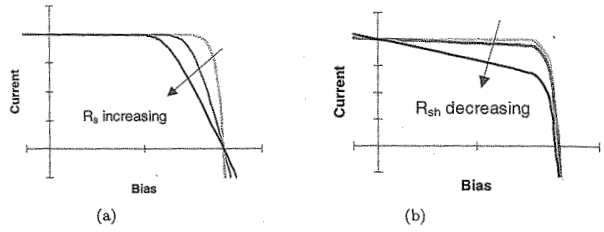
\includegraphics[width=\textwidth]{series_shunt_resistance.png}
    \caption{Effect of Series (a) and Shunt Resistance (b) on \ac{I-V} Curve}
    \label{fig:series_shunt_resistance}
\end{figure}

As shown in \autoref{fig:series_shunt_resistance} (b) from Nelson~\cite{nelson},
as the \acf{RSH} decreases, the top of the knee-bend of the \acf{I-V} curve will
be forced down. At low values of \ac{RSH} (on the order of $10$ $\si{\ohm}$),
the knee-bend will be pushed down so much that the curve becomes a straight
line. At high values of \ac{RSH}, (on the order of $100$ $\si{\ohm}$), the curve
converges to some fixed maximum bend constrained by other parameters of the
model. This relationship is generally considered logarithmic.

The \acf{ISH} can be added to the simple form of the model as a new term as
shown in \autoref{eq:cell_output_current_3}. Assuming that the \acf{RS} is
negligible ($0$), we can determine that \ac{ISH} is a function of the \ac{RSH}
and the \acf{VL}, as shown in \autoref{eq:cell_output_current_4}.

\begin{equation}
    I_L = I_{PV} - I_D - I_{SH}
    \equnit{\si{\ampere}}
    \label{eq:cell_output_current_3}
\end{equation}

\begin{equation}
    I_L = I_{PV} - I_D - \frac{V_L}{R_{SH}}
    \equnit{\si{\ampere}}
    \label{eq:cell_output_current_4}
\end{equation}


\subsection{Series Resistance}\label{subsec:five_param_series_resistance}

The \acf{RS} forces the knee-bend of the \ac{I-V} curve to the left or right, as
opposed to up and down for \ac{RSH}. As \ac{RS} increases, more current is
consumed across the lumped resistance before reaching the terminals of the solar
cell, reducing the expected current in the curve as shown in
\autoref{fig:series_shunt_resistance} (a). At high values of \ac{RS}, the curve
likewise becomes a straight line.

The \ac{RS} term impacts the consumers of the five parameter solar cell model;
namely the \ac{ID} and the \ac{RSH} terms. A visualization of this is shown as
\autoref{fig:current_junction}.

\begin{figure}[h]
    \centering
    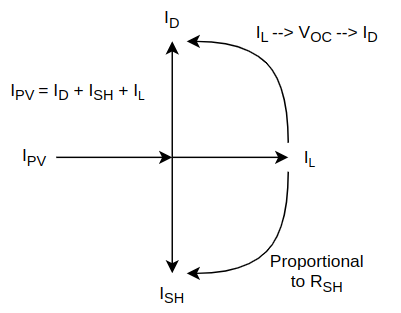
\includegraphics[width=0.7\textwidth]{cell_kirchoff_current_junction.png}
    \caption{Current Flow Junction of Five Parameter Model Solar Cell}
    \label{fig:current_junction}
\end{figure}

Revisiting \autoref{eq:cell_dark_current_1}, we know that the dark current
depends on \acf{VL} generated by \acf{IL} flowing through equivalent \acf{RL} connected at the cell
terminals. This allows us to reformulate the dark current equation as
\autoref{eq:cell_dark_current_2}. Here, we add the voltage drop across the
lumped series resistance summed with the \ac{VL} to represent the
total voltage expected by the dark current model.

\begin{equation}
    I_D = I_0[\exp(\frac{V_L + I_L R_S}{V_T}) - 1]
    \equnit{\si{\ampere}}
    \label{eq:cell_dark_current_2}
\end{equation}

We can likewise use the voltage drop to update the \ac{ISH} term, shown
in \autoref{eq:cell_shunt_current}.

\begin{equation}
    I_{SH} = \frac{V_L + I_L R_S}{R_{SH}}
    \equnit{\si{\ampere}}
    \label{eq:cell_shunt_current}
\end{equation}

Combining these two effects, we form \autoref{eq:cell_output_current_5}.

\begin{equation}
    I_{L} =  I_{PV} - I_0[\exp(\frac{V_L + I_L R_S}{V_T}) - 1] - \frac{V_L + I_L R_S}{R_{SH}}
    \equnit{\si{\ampere}}
    \label{eq:cell_output_current_5}
\end{equation}

We note that this model is an implicit function and cannot easily (or prettily)
move all the \ac{IL} terms to the left side of the equation. As such, for these
types of problems, we will develop and use iterative solvers to determine
\ac{IL} for a given set of input parameters (\ac{RS}, \ac{G}, \ac{VL}, etc).
Iterative solvers involve starting with a guess for the output parameter (in
this case \ac{IL}) and attempt to improve upon that guess such that each side is
equal to each other or within some tolerance to each other. An in depth
discussion on how these solvers were implemented for this model and variants of
this model can be found in \autoref{appendix:iterative_solvers}.

\todo[inline]{Augment appendix note with reference to
\ref{subsec:modeling_solar_cell_datasets}. Relegate appendix note to discussion
about iterative solvers and steps to build iterative solver (Desmos -> MATLAB ->
Python).}


\subsection{Photocurrent as a Ratio of Shunt/Series Resistance}\label{subsec:photocurrent_shunt_series_relation}

An interesting addition to the five parameter cell model is presented by Cubas
et al~\cite{cubas_et_al}\cite{cubas_et_al_2}: they observe that
\autoref{eq:cell_output_current_5} in short circuit conditions results in
\autoref{eq:cell_short_circuit_current_6}.

\begin{equation}
    I_{SC} = I_{PV} - I_0[\exp(\frac{I_{SC} R_S}{V_T}) - 1] - \frac{I_{SC} R_S}{R_{SH}}
    \equnit{\si{\ampere}}
    \label{eq:cell_short_circuit_current_6}
\end{equation}

In their analysis of measurements taken across a broad spectrum of reference
solar cells, represented in \autoref{table:dark_current_reference}, the dark
current at short circuit conditions were well less than a single milliampere, an
insignificant fraction of the total operating current. From this observation
Cubas et al. rewrites the above expression to get the photocurrent as a function
of \ac{ISC} and a ratio of \ac{RS} and \ac{RSH}, shown in
\autoref{eq:cell_photocurrent_3}.

\begin{equation}
    I_{PV} = I_{SC}\frac{R_S + R_{SH}}{R_{SH}}
    \equnit{\si{\ampere}}
    \label{eq:cell_photocurrent_3}
\end{equation}

\begin{table}[h!]
    \begin{tabularx}{\textwidth}{
        | >{\raggedright\arraybackslash}X
        | >{\raggedright\arraybackslash}X
        | >{\raggedright\arraybackslash}X
        | >{\raggedright\arraybackslash}X
        | >{\raggedright\arraybackslash}X | }
        \hline
        Reference & Cell Type & \ac{ISC} (A) & $I_0[e^{\frac{I_{SC} R_S}{V_T}} -
        1]$ (A) & \ac{ID} / \ac{ISC} \\ \hline \hline
        Kennerud, 1969  & CdS   & 0.8040 & 1.56E-5 & 1.94E-5 \\ \hline
        Charles, 1981   & BSC   & 0.1023 & 2.21E-8 & 2.16E-7 \\ \hline
        Charles, 1981   & GSC   & 0.5610 & 1.01E-5 & 1.80E-5 \\ \hline
        Lo Brano, 2010  & Q6LM  & 7.6650 & 1.42E-9 & 1.85E-10 \\ \hline
    \end{tabularx}
    \caption{Dark Current Ratios for Various Reference Cells}
    \label{table:dark_current_reference}
\end{table}

However, a cursory evaluation of the parameter space (\ac{VOC}, \ac{ISC},
\ac{G}, \ac{TC}, \ac{RS}, \ac{N}) reveals that the assumption that the dark
current is negligible breaks down when a subset of the following conditions
occur:

\begin{itemize}
    \item the \acf{VOC} becomes very small,
    \item the \acf{ISC} becomes very large,
    \item and the \acf{RS} becomes relatively large for some
    combination of \ac{VOC} and \ac{ISC}.
\end{itemize}

Is it to be noted that these parameters are tightly coupled, and therefore the
language specifying a parameter space upon which this term should be used
remains imprecise. We also note that \ac{TC} and \ac{N} when increased slightly
tighten the viable parameter space.

However, when considering a specific solar cell that is \textit{appropriate}
(e.g.\ it contains \ac{STC} defined parameters \ac{VOC} and \ac{ISC} with an
measured \ac{RS} that results in negligible \ac{ID}), this term remains
negligible unless the cell is exposed to (1) high temperatures or (2) high
intensity light, two conditions that tend to come hand in hand. These conditions
tend to only be experienced by concentrator photovoltaics and are highly
unlikely to be reached by normal solar cells.

We will observe later in \autoref{sec:evaluation_of_solar_module_models} that
with our dataset of Maxeon Gen III Bin Le1 solar cells, the vast majority of
estimated series resistance is well below $0.08 \si{\ohm}$, which results in
dark currents less than a m\si{\ampere}. This means that this modification
(assuming it improves the accuracy of the model), is well suited for our solar
cells.

Incorporating this revision, we arrive at \autoref{eq:cell_short_circuit_current_7}.

\begin{equation}
    I_L = I_{SC}\frac{R_S + R_{SH}}{R_{SH}} - I_0[\exp(\frac{V_L + I_L R_S}{V_T}) - 1] - \frac{V_L + I_L R_S}{R_{SH}}
    \equnit{\si{\ampere}}
    \label{eq:cell_short_circuit_current_7}
\end{equation}

\todo[inline]{See \url{https://www.desmos.com/calculator/nniw0mha2k} to play
around with the revised dark current model. Add as a figure later on compared to
experimental data.}


\subsection{Shunt and Series Resistance as a Function of Irradiance, Temperature}\label{subsec:rsh_rs_dependence}

Throughout this major section, we introduced the notion of shunt and series
resistance as internal parasitics. However, we did not explore whether these
`internal parameters' are themselves affected by external conditions such as
irradiance and temperature.

A comprehensive review and experimental paper from Fébba et
al~\cite{febba_et_al} performed experiments on solar cells to evaluate the
effect of temperature and irradiance on shunt and series resistance, controlling
for the two independent variables in ranges of $25\si{\celsius}$ to
$55\si{\celsius}$ and $600\si{\watt/\meter^2}$ to $1000\si{\watt/\meter^2}$,
respectively. Four figures,
\autoref{fig:febba_shunt_resistance_and_temperature}~-~\autoref{fig:febba_series_resistance_and_irradiance}
are shown below to illustrate the following assertions.

For \acf{RSH}, they observed the following trends:

\begin{itemize}
    \item as temperature increases, the \ac{RSH} exponentially decays,
    \item and as irradiance increases, the \ac{RSH} linearly decreases.
\end{itemize}

For \ac{RS}, they observed the following trends:

\begin{itemize}
    \item as temperature increases, the \ac{RS} exponentially decays,
    \item and as irradiance increases, the \ac{RS} linearly increases.
\end{itemize}

\begin{figure}[!htbp]
    \centering
    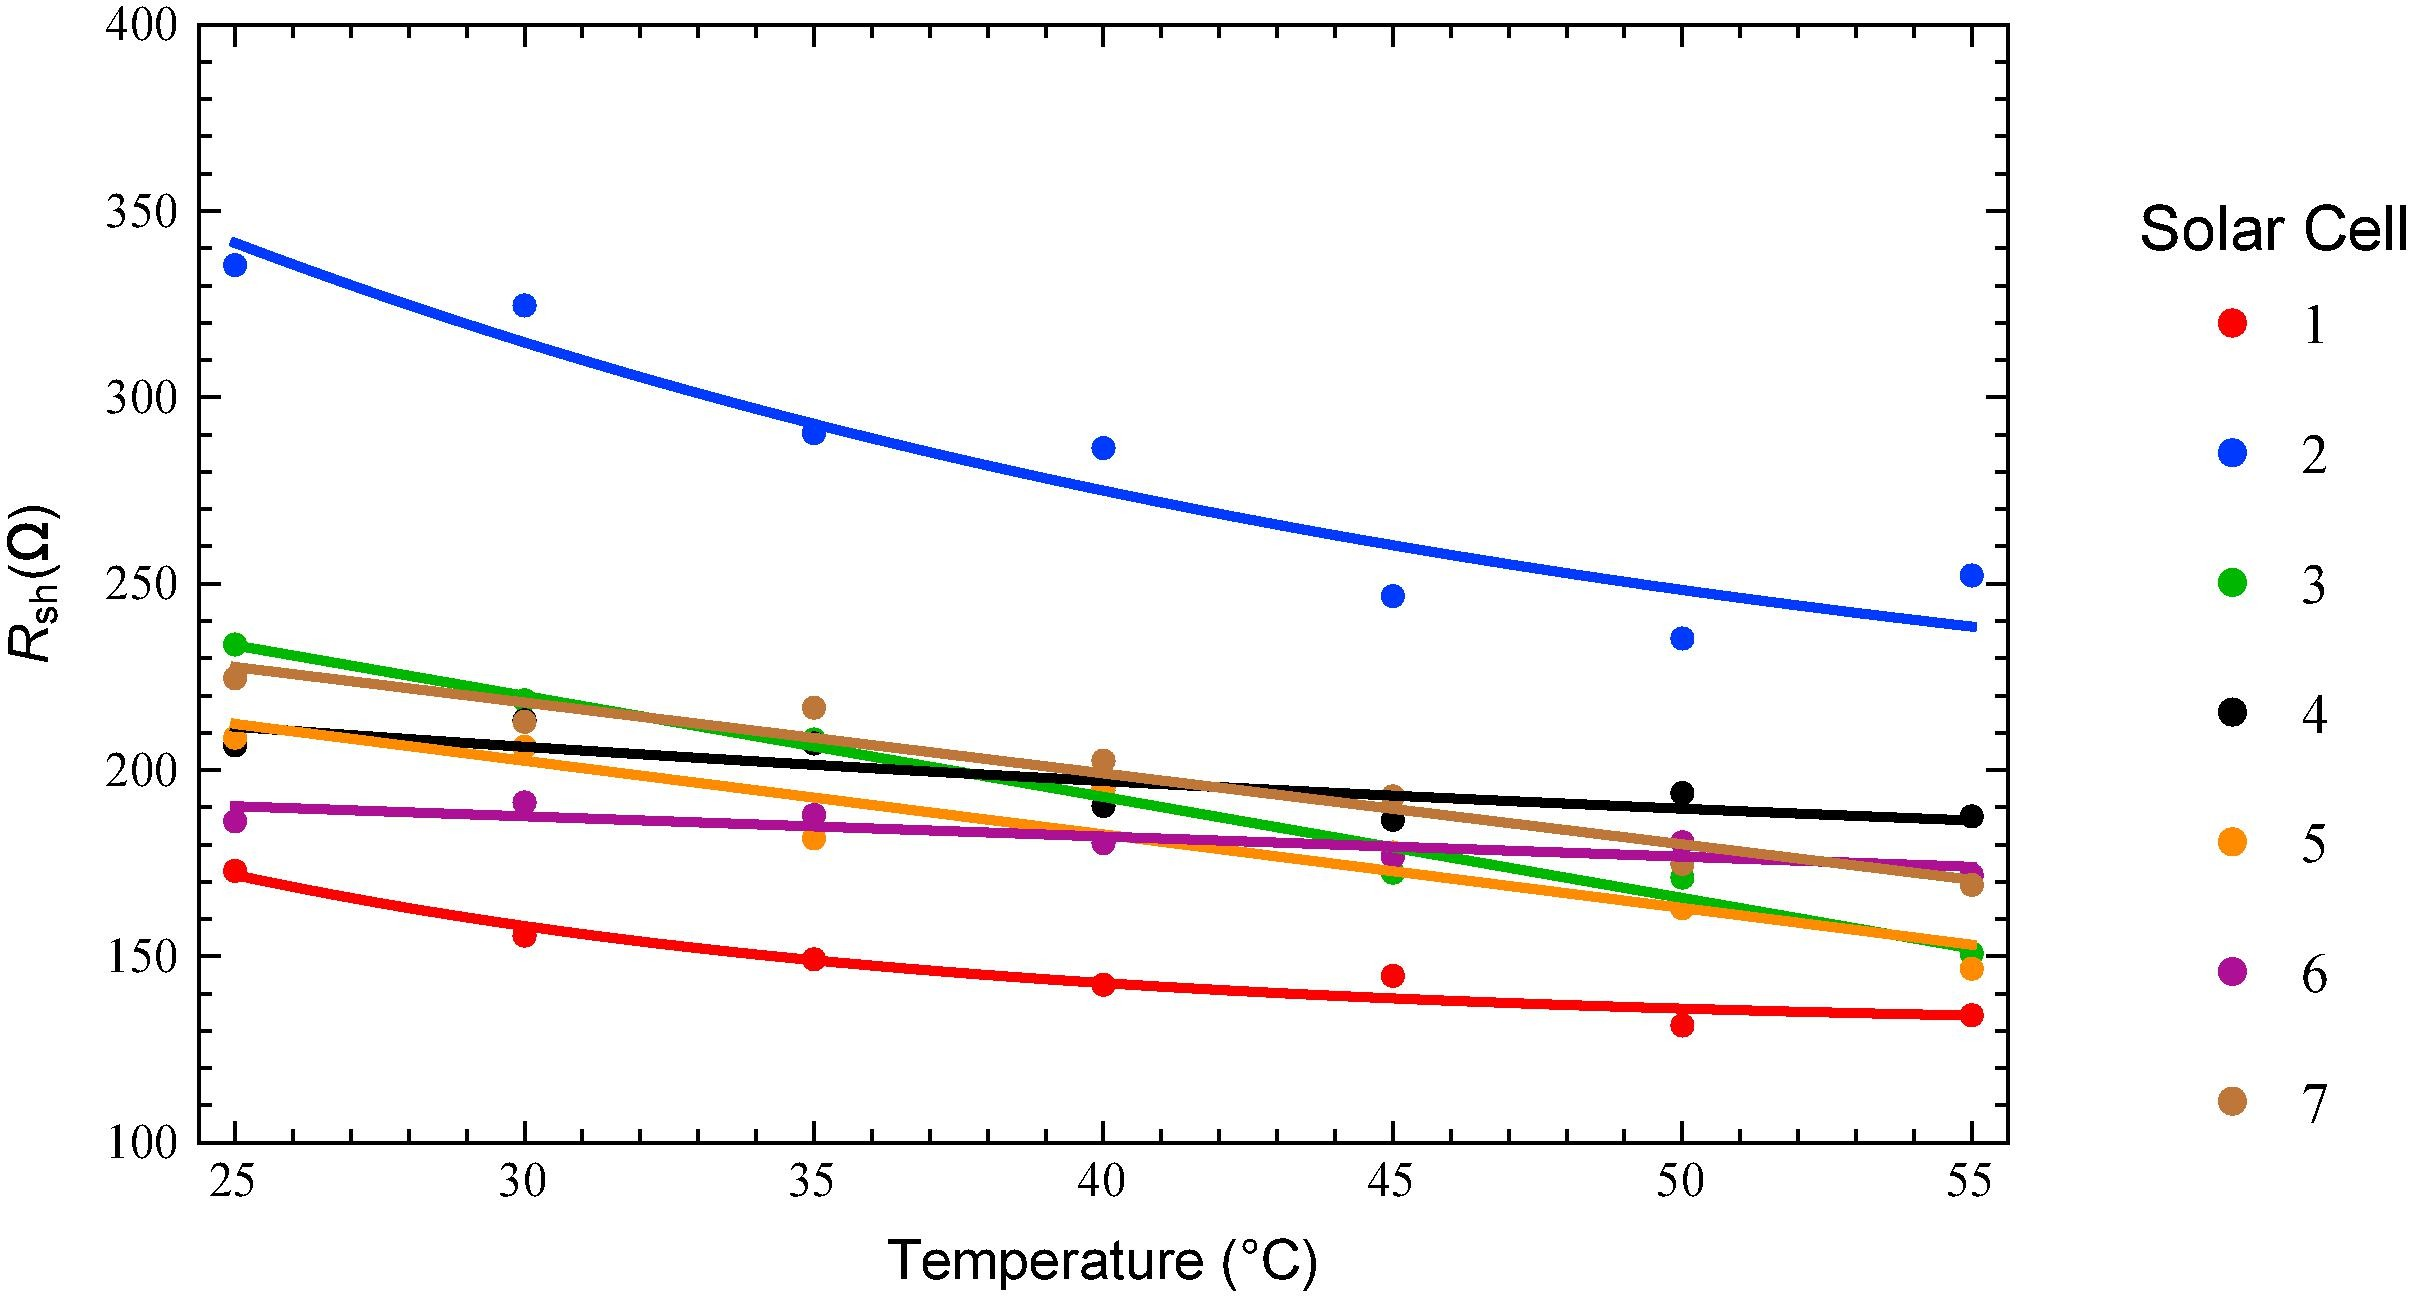
\includegraphics[width=0.75\textwidth]{febba_shunt_resistance_and_temperature.jpg}
    \caption{Shunt Resistance vs Temperature~\cite{febba_et_al}}
    \label{fig:febba_shunt_resistance_and_temperature}
\end{figure}

\begin{figure}[!htbp]
    \centering
    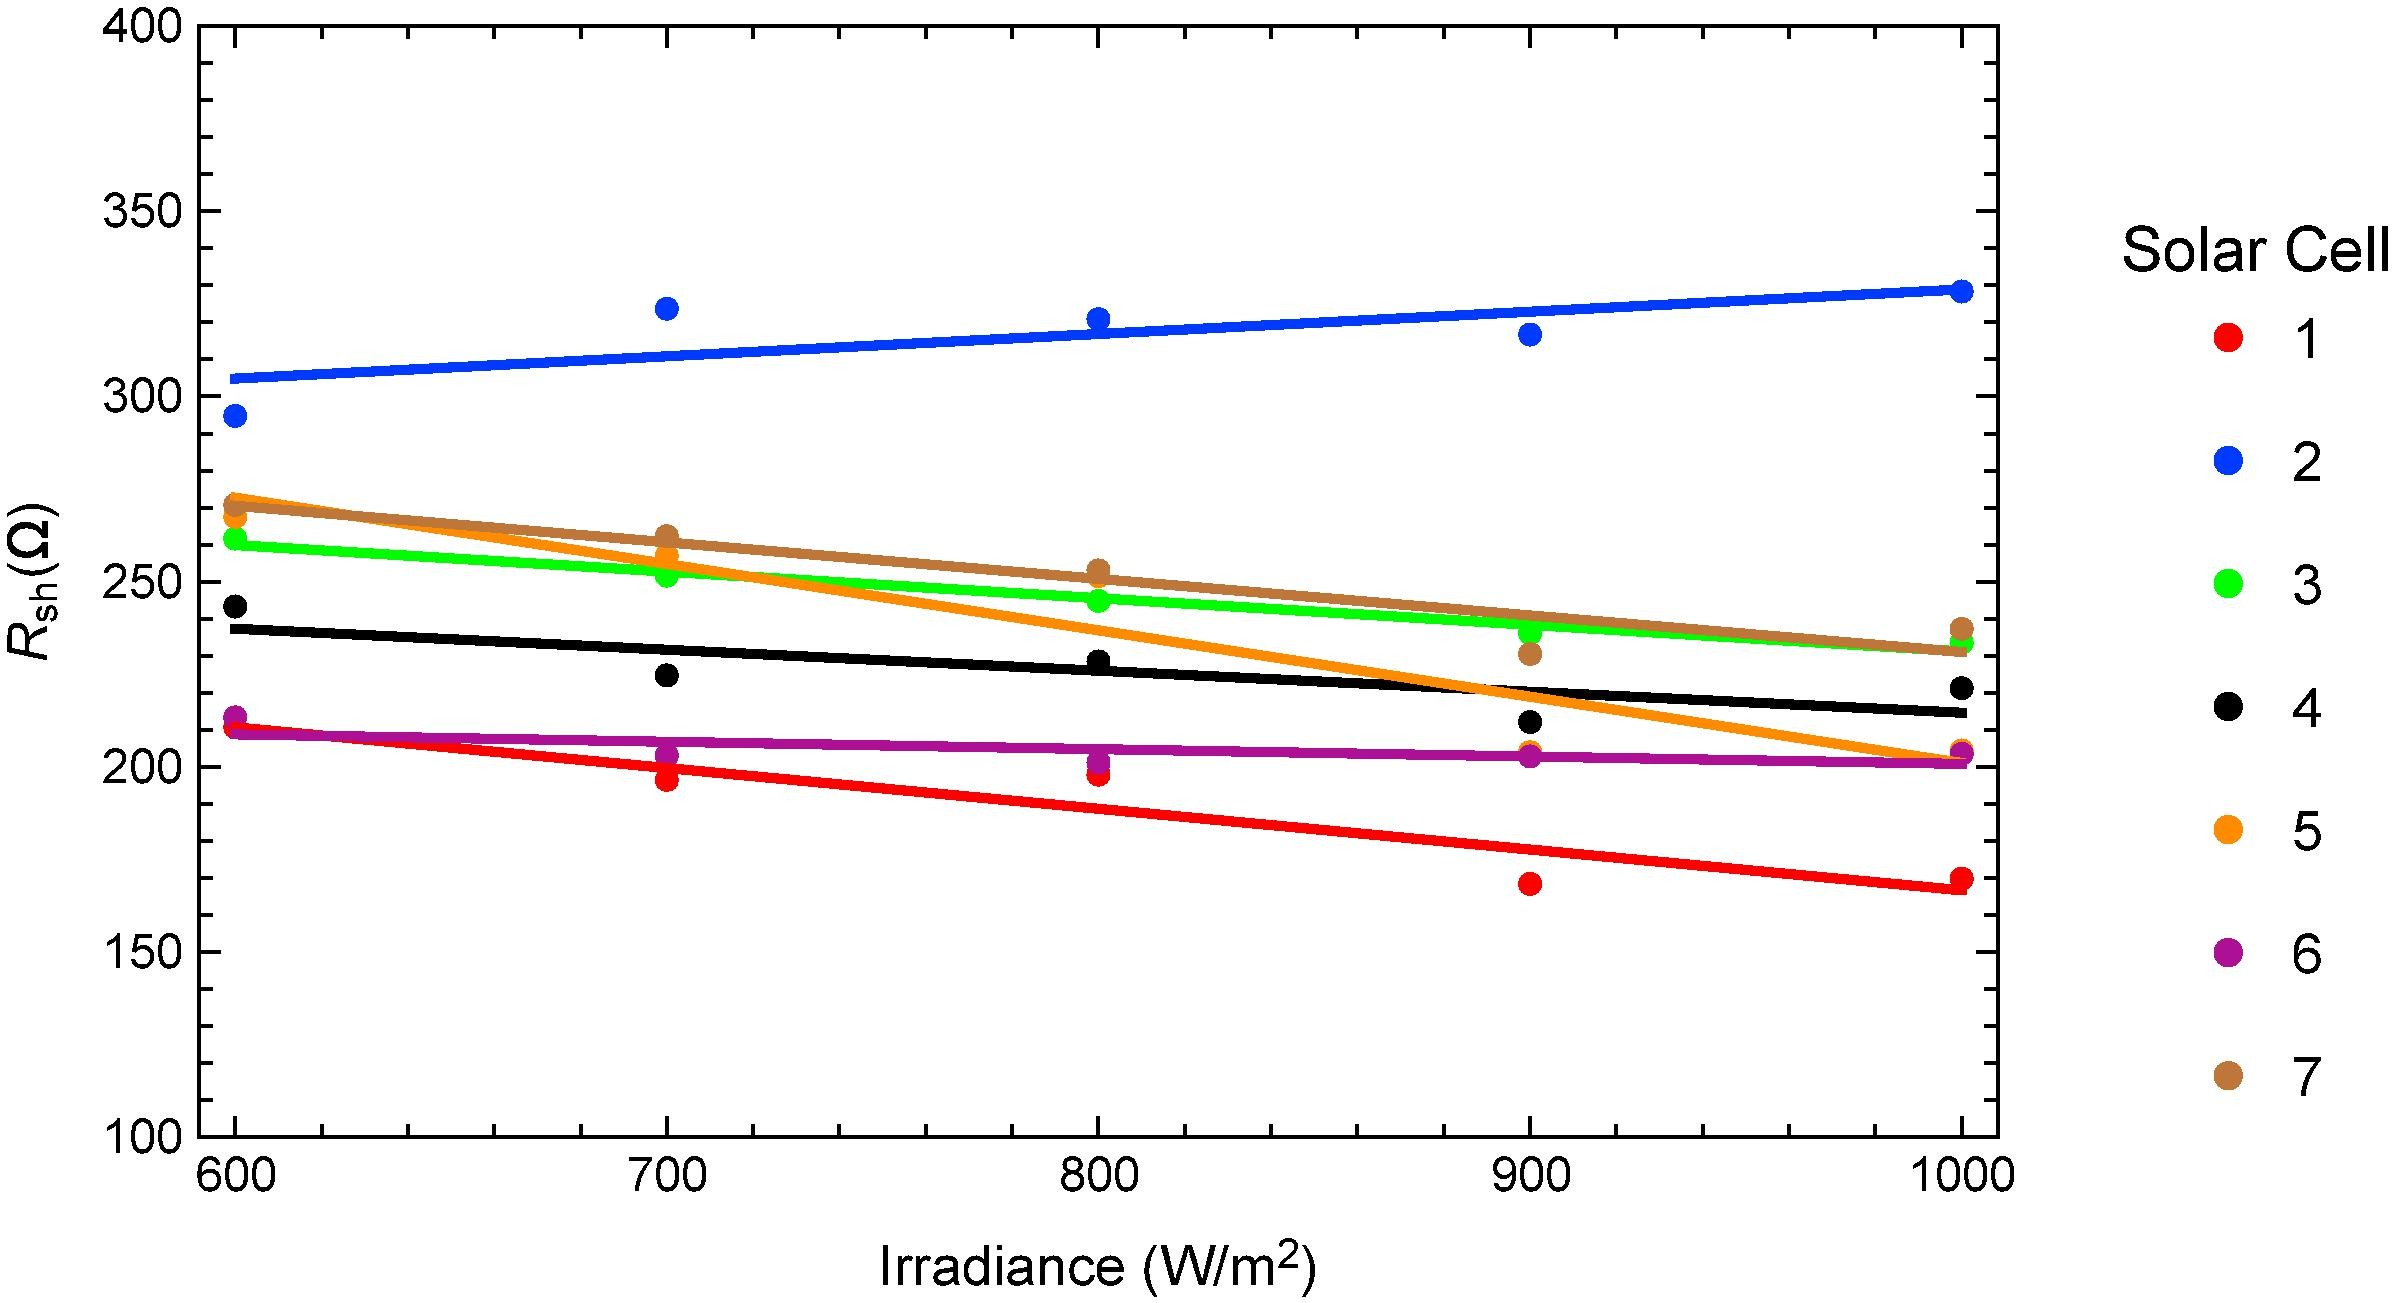
\includegraphics[width=0.75\textwidth]{febba_shunt_resistance_and_irradiance.jpg}
    \caption{Shunt Resistance vs Irradiance~\cite{febba_et_al}}
    \label{fig:febba_shunt_resistance_and_irradiance}
\end{figure}

\begin{figure}[!htbp]
    \centering
    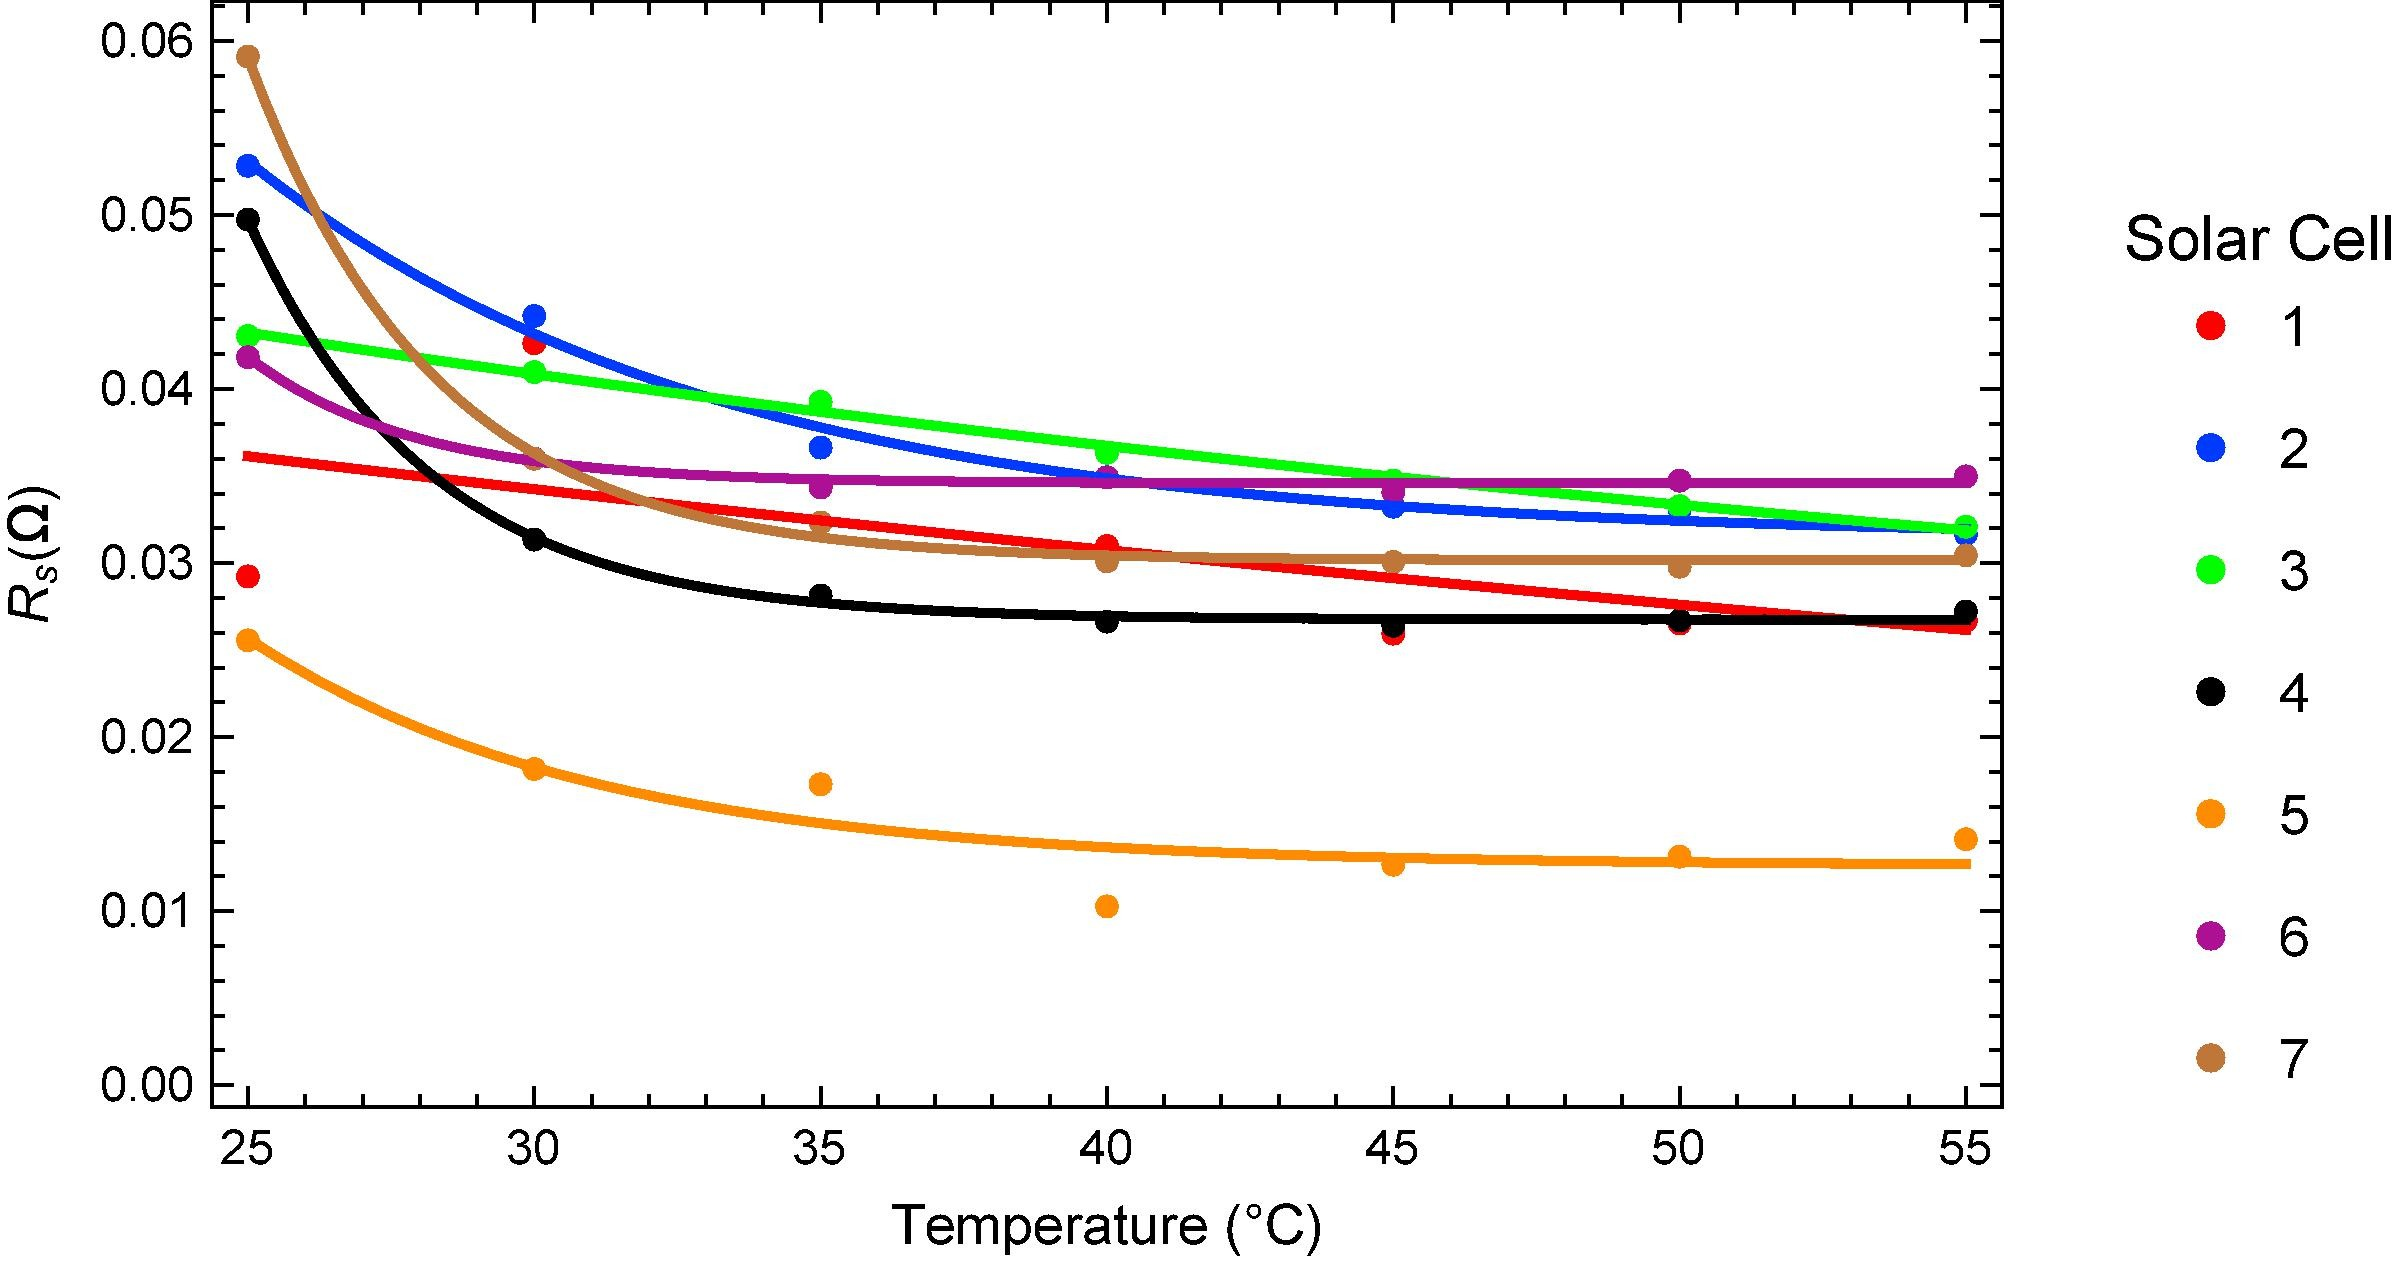
\includegraphics[width=0.75\textwidth]{febba_series_resistance_and_temperature.jpg}
    \caption{Series Resistance vs Temperature~\cite{febba_et_al}}
    \label{fig:febba_series_resistance_and_temperature}
\end{figure}

\begin{figure}[!htbp]
    \centering
    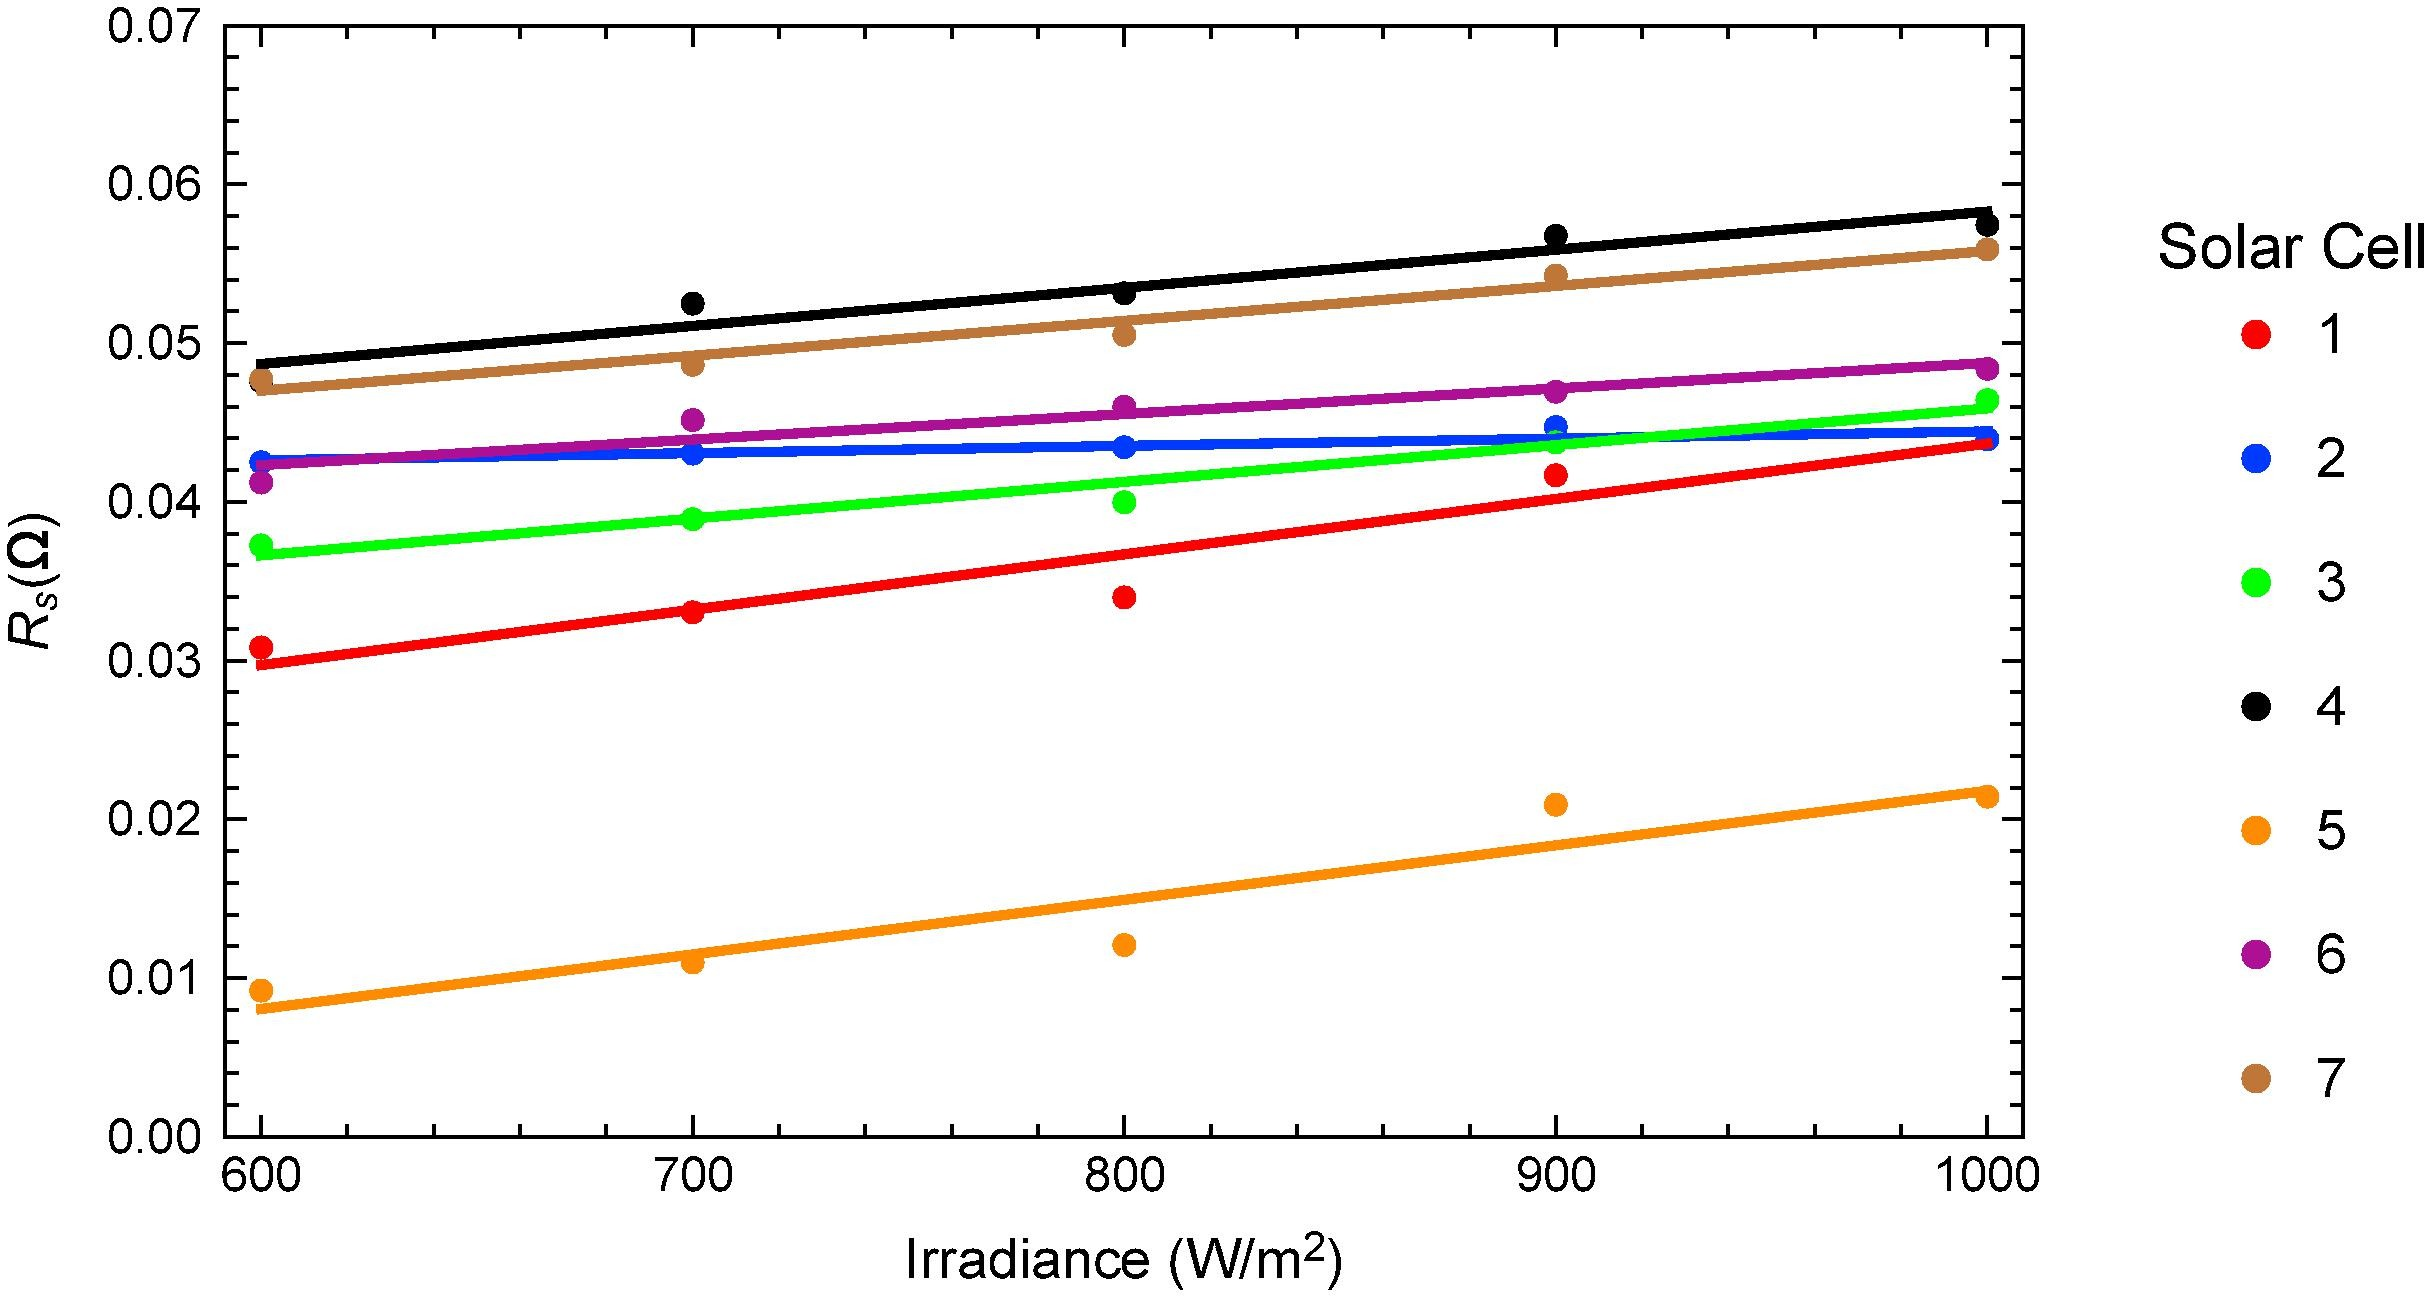
\includegraphics[width=0.75\textwidth]{febba_series_resistance_and_irradiance.jpg}
    \caption{Series Resistance vs Irradiance~\cite{febba_et_al}}
    \label{fig:febba_series_resistance_and_irradiance}
\end{figure}

Fébba et al. did not posit a revised model of the either resistance term
(although they did provide explanations on why the trends were reasonable), but
Baig et al.~\cite{baig_et_al} and MacAlpine et
Brandemuehl~\cite{macalpine_et_brandemuehl} introduced a variant of
\autoref{eq:series_resistance_1} that uses a \ac{ZETA}.

\begin{equation}
    R_S = R_{S,ref} \exp(\zeta [T_{C,ref} - T_C])
    \equnit{\si{\ohm}}
    \label{eq:series_resistance_1}
\end{equation}

We extend Fébba et al~\cite{febba_et_al}'s results to generate
\autoref{eq:series_resistance_2}, adding a \ac{ETA}, applied to
\autoref{eq:series_resistance_1}.

\begin{equation}
    R_S = R_{S,ref} \exp(\zeta [T_{C,ref} - T_C])[1 + \eta(G_{ref} - G)]
    \equnit{\si{\ohm}}
    \label{eq:series_resistance_2}
\end{equation}

We also propose \autoref{eq:shunt_resistance} to model the shunt
resistance, with \ac{KAPPA} and \ac{IOTA}.

\begin{equation}
    R_{SH} = R_{SH,ref} \exp(\kappa [T_{C,ref} - T_C])[1 + \iota [G_{ref} - G]]
    \equnit{\si{\ohm}}
    \label{eq:shunt_resistance}
\end{equation}

We also note that a solar cell consists of a network of resistors and diodes. If
we dispel the assumptions that the solar cell is (a) entirely and evenly
illuminated, (b) uniformly heated, and (c) of consistent manufacturing quality,
the apparent series resistance measured at the terminals of the cell can
fluctuate. An example of this is provided below in
\autoref{fig:cell_with_varying_series_resistance}. Depending on the
proportion of the solar cell with varying amounts of series resistance, the
observed \ac{I-V} curve could differ greatly.

\begin{figure}[h]
    \centering
    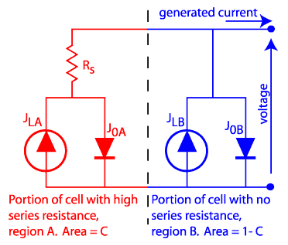
\includegraphics[width=0.5\textwidth]{cell_with_varying_series_resistance.png}
    \caption{Solar Cell With Varying Series Resistances~\cite{pveducation_measurement_of_series_resistance}}
    \label{fig:cell_with_varying_series_resistance}
\end{figure}

Replication of Fébba et al's work is presented in
\autoref{appendix:parasitics_measurements}, where a custom testbed is used
to measure solar cell curves at various temperature and irradiance levels at a
broader range compared to Fébba et al ($0\si{\celsius}$ to $100\si{\celsius}$
and $0\si{\watt/\meter^2}$ to $1000\si{\watt/\meter^2}$, respectively).
Additionally, \autoref{appendix:parasitics_measurements} also discusses
methods to evaluate the resistances and their respective coefficients. The
evaluation of the effectiveness of these terms in predicting the expected
\ac{I-V} curves warrants their own subsection in
\autoref{sec:evaluation_of_solar_cell_models}.

\todo[inline]{Augment appendix note with reference to
\ref{subsec:experimental_extraction_of_cell_parameters}. Relegate appendix note
with in depth experimental measurements and statistics.}


\subsection{Model Summary}\label{subsec:five_param_model_summary}

To conclude this major section, we will review the components that make up the
five parameter cell model, propose an item of further exploration, and propose a
complete model function that incorporates the topics discussed.

Firstly, the five parameter cell model retains the attributes of the three
parameter cell model, being the complete form of the single diode model. It adds
two parameters, a \acf{RSH} and \acf{RS} that represent ohmic losses in the
solar cell, which primarily affect the knee-bend of the resultant \ac{I-V}
curve. These two parameters help reduce error in the model around the knee-bend
that cannot fully be represented by the ideality factor. However, these
additions increase the complexity of the model, and the resultant form is an
implicit equation that requires an iterative solver approach.

Secondly, we investigate a revision to the photocurrent model to make it also a
function of \ac{RS} and \ac{RSH}. This was obtained by evaluating the short
circuit condition of the existing model and reducing the dark current term under
appropriate conditions. We note that this new model may not work under specific
conditions, namely for concentrator solar cells or for solar cells with
inordinately large series resistance relative to their specific \ac{VOC} and
\ac{ISC} combination.

We also discuss evaluating \ac{RS} and \ac{RSH} themselves as a function of
temperature and irradiance. We observe that these values tend to have
exponential relationships with temperature and linear relationships with
irradiance, although we require further data to validate the strength of these
correlations. We derive initial models for these parameters, and discuss real
world conditions in which they might deviate from our expectations (e.g. partial
shading).

As such, we will revisit both of these modifications to the base model in a
further section to prove or disprove their veracity and usefulness to the
overall model.

Finally, we incorporate these changes into the complete function defined in the
previous section. This is presented as \autoref{eq:cell_output_current_6}
(\ac{ISC}, \ac{VOC}, \ac{RS}, \ac{RSH}, and \ac{VT} abstracted out for clarity
and brevity). We observe that this complete model builds upon the existing
parameters named in \autoref{subsec:three_param_model_summary} by adding two
extra reference parameters:

\begin{itemize}
    \item \acf{RSREF}
    \item \acf{RSHREF}
\end{itemize}

and four more curve fitting parameters:

\begin{itemize}
    \item \acf{ZETA}
    \item \acf{ETA}
    \item \acf{KAPPA}
    \item \acf{IOTA}
\end{itemize}

For the cells tested in this project, the reference parameters \ac{RSREF} and
\ac{RSHREF} were evaluated from the data empirically. Like \acf{N} and
\acf{ZETA}, the curve fitting parameters must be derived from curve fitting
technique or other statistical methods (such as building a distribution of cells
at various irradiances to calculate a generic coefficient subject to the
\ac{CLT}).

\todo{Reformat this equation}
\begin{equation}
    \begin{split}
        I_L(V_L, G, T_C) &= I_{PV}(G, T_C, R_S, R_{SH}) - I_D(V_L, G, T_C, R_S) - I_{SH}(R_S, R_{SH}) \\
        & = I_{SC}(G, T_C)\frac{R_S + R_{SH}}{R_{SH}} - I_0(G, T_C)[\exp(\frac{V_L + I_L R_S}{V_T(T_C)}) - 1] - \frac{V_L + I_L R_S}{R_{SH}} \\
        & = I_{SC}(G, T_C)\frac{R_S + R_{SH}}{R_{SH}} - I_{SC}(G, T_C)\frac{\exp(\frac{V_L + I_L R_S}{V_T(T_C)}) - 1}{\exp(\frac{V_{OC}(G, T_C)}{V_T(T_C)}) - 1} - \frac{V_L + I_L R_S}{R_{SH}} \\
        & = I_{SC}(G, T_C)[\frac{R_S + R_{SH}}{R_{SH}} + \frac{1 - \exp(\frac{V_L + I_L R_S}{V_T(T_C)})}{1 - \exp(\frac{V_{OC}(G, T_C)}{V_T(T_C)})}] - \frac{V_L + I_L R_S}{R_{SH}}
    \end{split}
    \equnit{\si{\ampere}}
    \label{eq:cell_output_current_6}
\end{equation}

\todo[inline]{See \url{https://www.desmos.com/calculator/yp0rhmabkz} to play
around with the complete three parameter solar cell model. Add as a figure later
on compared to experimental data.}

\newpage
\section{Seven Parameter Solar Cell Model}\label{sec:seven_parameter_solar_cell_model}

\subsection{Model Introduction}\label{subsec:seven_param_model_introduction}

\begin{figure}[h]
    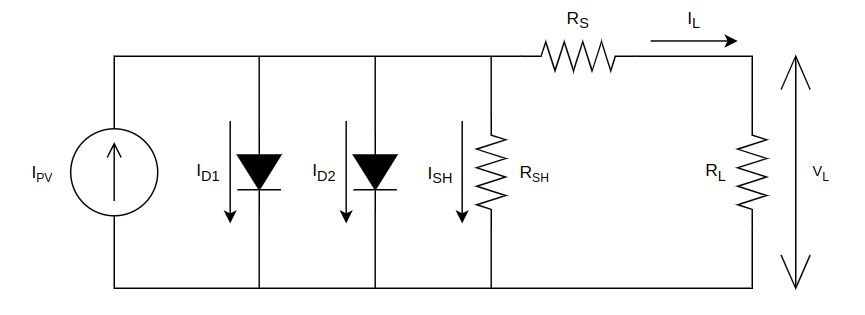
\includegraphics[width=\textwidth]{solar_cell_seven_parameter_model.png}
    \caption{Seven Parameter, or Double Diode Model of a Solar Cell}
    \label{fig:double_diode_model}
\end{figure}

The seven parameter solar cell model, also known as a double diode model, shown
in \autoref{fig:double_diode_model}, builds upon the five parameter model by
introducing a second diode (hence the name) to more accurately model internal
current losses, which can be split into the following:

\begin{itemize}
    \item losses due to carrier recombination in the space charge region of the
    P-N junction,
    \item and losses due to surface recombination.
\end{itemize}

These currents are denoted as \acf{ID1} and \acf{ID2}, respectively. By
differentiating between the two primary recombination processes in the cell, the
seven parameter model is generally considered more accurate than the five
parameter model.

The general form of this equation is shown in \autoref{eq:cell_output_current_7}.

\begin{equation}
    I_L = I_{PV} - I_{D1} - I_{D2} - I_{SH}
    \equnit{\si{\ampere}}
    \label{eq:cell_output_current_7}
\end{equation}

This results in the \autoref{eq:cell_output_current_8} when all components have
been inserted:

\begin{equation}
    \begin{split}
        I_L(V_L, G, T_C) &= I_{PV}(G, T_C, R_S, R_{SH})
                          - I_{D1}(V_L, G, T_C, R_S)
                          - I_{D2}(V_L, G, T_C, R_S) \\
        & \quad           - I_{SH}(R_S, R_{SH}) \\
        &                 = I_{SC}(G, T_C)\frac{R_S + R_{SH}}{R_{SH}}
                          - I_{01}(G, T_C)[\exp(\frac{q[V_L + I_L R_S]}{n_1 k_B T_C}) - 1] \\
        & \quad           - I_{02}(G, T_C)[\exp(\frac{q[V_L + I_L R_S]}{n_2 k_B T_C}) - 1]
                          - \frac{V_L + I_L R_S}{R_{SH}} \\
        &                 = I_{SC}(G, T_C)\frac{R_S + R_{SH}}{R_{SH}}
                          - I_{SC}(G, T_C)\frac{\exp(\frac{q[V_L + I_L R_S]}{n_1 k_B T_C}) - 1}{\exp(\frac{qV_{OC}(G, T_C)}{n_1 k_B T_C}) - 1} \\
        & \quad           - I_{SC}(G, T_C)\frac{\exp(\frac{q[V_L + I_L R_S]}{n_2 k_B T_C}) - 1}{\exp(\frac{qV_{OC}(G, T_C)}{n_2 k_B T_C}) - 1}
                          - \frac{V_L + I_L R_S}{R_{SH}} \\
        &                 = I_{SC}(G, T_C)[
                                \frac{R_S + R_{SH}}{R_{SH}}
                              + \frac{1 - \exp(\frac{q[V_L + I_L R_S]}{n_1 k_B T_C})}{1 - \exp(\frac{qV_{OC}(G, T_C)}{n_1 k_B T_C})} \\
        & \quad               + \frac{1 - \exp(\frac{q[V_L + I_L R_S]}{n_2 k_B T_C})}{1 - \exp(\frac{qV_{OC}(G, T_C)}{n_2 k_B T_C})}]
                          - \frac{V_L + I_L R_S}{R_{SH}}
    \end{split}
    \equnit{\si{\ampere}}
    \label{eq:cell_output_current_8}
\end{equation}

We note in this equation \ac{VT} was substituted back in to demonstrate that
each ideality constant for each diode is unique.

\newpage
\todo[inline]{Behold! True evil!!!\newline Not for general consumption.}
\begin{equation}
    \begin{split}
        I_L(V_L, G, T_C) &= I_{SC,ref}\frac{G}{G_{ref}}[1 - \alpha(T_{C,ref} - T_C)] \\
        & \quad             [ \\
        & \quad\quad            \frac{R_{S,ref} \exp(\zeta [T_{C,ref} - T_C])[1 + \eta(G - G_{ref})]}{R_{SH,ref} \exp(\kappa [T_{C,ref} - T_C])[1 - \iota(G - G_{ref})]} + 1 \\
        & \quad\quad          + \frac{1 - \exp(\frac{q[V_L + I_L R_{S,ref} \exp(\zeta [T_{C,ref} - T_C])[1 + \eta(G - G_{ref})]]}{n_1 k_B T_C})}{1 - \exp(\frac{q[V_{OC,ref}[1 - \beta (T_{C,ref} - T_C)] + \frac{nk_B(T_{C,ref} + T_C/\gamma)}{q}\ln(\frac{G}{G_{ref}})](G, T_C)}{n_1 k_B T_C})} \\
        & \quad\quad          + \frac{1 - \exp(\frac{q[V_L + I_L R_{S,ref} \exp(\zeta [T_{C,ref} - T_C])[1 + \eta(G - G_{ref})]]}{n_2 k_B T_C})}{1 - \exp(\frac{q[V_{OC,ref}[1 - \beta (T_{C,ref} - T_C)] + \frac{nk_B(T_{C,ref} + T_C/\gamma)}{q}\ln(\frac{G}{G_{ref}})](G, T_C)}{n_2 k_B T_C})} \\
        & \quad             ] \\
        & \quad             - \frac{V_L + I_L R_{S,ref} \exp(\zeta [T_{C,ref} - T_C])[1 + \eta(G - G_{ref})]}{R_{SH,ref} \exp(\kappa [T_{C,ref} - T_C])[1 - \iota(G - G_{ref})]}
    \end{split}
    \equnit{\si{\ampere}}
    \label{eq:cell_output_current_9}
\end{equation}

\subsection{Model Summary}\label{subsec:seven_param_model_summary}

\todo[inline]{Might want to look for some more novel content, or wrap this section up as
is. Nothing particularly new here besides another parameter to estimate.}

\newpage
\section{Evaluation of Solar Cell Models}\label{sec:evaluation_of_solar_cell_models}

To evaluate these solar cell models and their proposed modifications, we used a
set of almost 450 Maxeon Gen III and Maxeon C60 solar cells. In this section, we
will discuss the aspects of this collection, how we characterized the solar
cells to generate a robust dataset with custom \acf{HW} and \acf{SW}, and
techniques (both experimental and statistical) to evaluate and estimate their
parameters. Finally, we'll use these parameters to compare the models and their
real world equivalents to determine model accuracy and precision.


\subsection{Solar Cell Dataset}\label{subsec:solar_cell_dataset}

The solar cells used for the \ac{LHRs} solar vehicle are a mixture of Maxeon Gen
III and Maxeon C60 solar cells. These solar cells were selected primarily due to
financial and availability constraints; historically, in the last two solar
vehicle revisions (2018, 2021) Gen III Bin Le1 cells have been used, but this
year the team decided to procure cheaper, more easily available C60 cells from
secondary suppliers. Regardless, both of these cell lines remain state of the
art despite their age \footnote{dates are unclear, but it appears that C60 was
introduced around 2007\cite{sunpower_history} and the Gen III has been around as
long as 2013\cite{smith_et_al}.}; both Aptera Motors\cite{aptera_solar_cells}
and Lightyear One\cite{lightyear_one_solar_cells} -the latter of which is a
former Solar Vehicles team- have announced cooperation with Maxeon to use their
solar cells. Aptera in particular uses the Gen III
cells\cite{aptera_solar_cells}.

While these cell types are both $125 \si{\mm}$ by $125 \si{mm}$ (see
\autoref{fig:maxeon_gen_iii_cell_footprint} for a visualization of the cell
physical layout), the Gen III cells are slightly more efficient than the C60
cells. Their (Gen III) rear contacts also tend to be slightly narrower than the
C60 cells. Their electrical characteristics are outlined in
\autoref{fig:maxeon_gen_iii_cell_characteristics} and
\autoref{fig:maxeon_c60_cell_characteristics}. Note that the Maxeon Gen III
cells are explicitly Bin Le1 cells, although the dataset will later show that
the binning for both groups of cells tends to not be very respective of the
actual measured \ac{I-V} curves, which is likely due to the variance in our
testing setup.

Since these cells were unpacked and designated for specific years,
\autoref{table:solar_cell_dataset} is provided to delineate between the
different types and `lines' of cells tested. `Lines' in this sense indicate
the academic year the cells were originally unpacked and tested.

\begin{figure}[!htbp]
    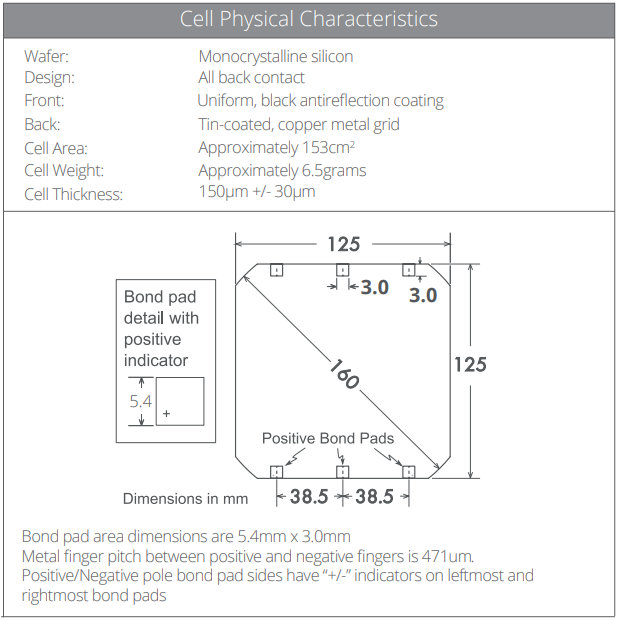
\includegraphics[width=\textwidth]{maxeon_gen_iii_cell_footprint.png}
    \caption{Maxeon Gen III Cell Footprint}
    \label{fig:maxeon_gen_iii_cell_footprint}
\end{figure}

\begin{figure}[!htbp]
    \centering
    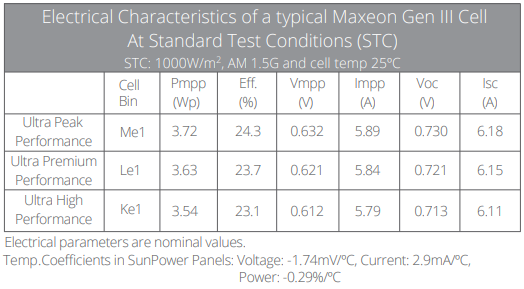
\includegraphics[width=0.8\textwidth]{maxeon_gen_iii_cell_characteristics.png}
    \caption{Maxeon Gen III Cell Characteristics}
    \label{fig:maxeon_gen_iii_cell_characteristics}
\end{figure}

\begin{figure}[!htbp]
    \centering
    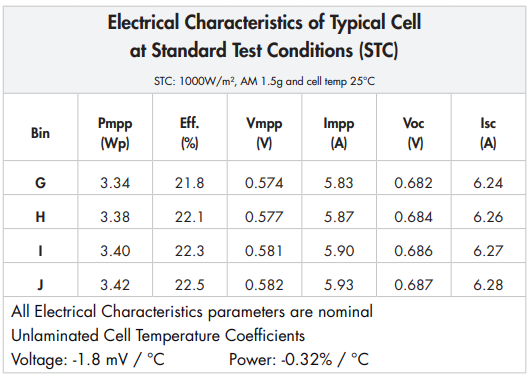
\includegraphics[width=0.8\textwidth]{maxeon_c60_cell_characteristics.png}
    \caption{Maxeon C60 Cell Characteristics}
    \label{fig:maxeon_c60_cell_characteristics}
\end{figure}

\begin{table}[!htbp]
    \begin{tabularx}{\textwidth}{
        | >{\raggedright\arraybackslash}X
        | >{\raggedright\arraybackslash}X
        | >{\raggedright\arraybackslash}X
        | >{\raggedright\arraybackslash}X | }
        \hline
        Cell Line   & Year Unpacked & Type      & Number of Cells \\ \hline \hline
        RP          & 2022          & C60       & X               \\ \hline
        MW          & 2020          & Gen III   & X               \\ \hline
        2019\_Le1   & 2019          & Gen III   & X               \\ \hline
        BU          & 2018          & Gen III   & X               \\ \hline
    \end{tabularx}
    \caption{Cell Lines Used in Solar Cell Dataset}
    \label{table:solar_cell_dataset}
\end{table}
\todo[inline]{Add number of cells tested to each group in table.}


\subsection{Characterizing Solar Cells}\label{subsec:characterizing_solar_cells}

\todo[inline,caption={}]{
    \begin{itemize}
        \item Introduction to proposed testing setup (add image)
        \item Discussion of light source,
        https://www.mpja.com/download/34769opdata.pdf MPJA grow lights, spectrum
        \item Discussion of irradiance control, Blackbody C (refer to Appendix C)
        \item Discussion of how to measure the solar cell (refer to Appendix D)
        \item Process of characterizing solar cell (assembly, test, disassembly)
    \end{itemize}
}

To characterize solar cells, we develop a test setup as outlined in
\autoref{fig:cell_test_setup}. In this test setup, we maintain three critical
requirements:

\begin{itemize}
    \item The test article shall receive a \textit{measurable} and
    \textit{consistent} irradiance over the test duration.
    \item The test article shall receive a \textit{uniform} irradiance over the
    span of the test article.
    \item The test article shall maintain a \textit{measurable} and
    \textit{consistent} surface temperature over the test duration.
\end{itemize}

To achieve these aforementioned requirements, a solar cell or solar module of up
to $500 \si{\mm}$ by $250 \si{mm}$ (equivalent to 4 cells by 2 cells) in size is
placed upon a thermal bed separated by a thin, electrically insulating layer of
Kapton tape; the photovoltaic is maintained at a fixed temperature by the
thermal bed through conduction, which is controlled by a \todo{Insert name of
heater/ chiller device} XXX. A solar simulator, consisting of a set of dimmable
grow light modules (MPJA 34769-OPs), is mounted to an aluminum plate heatsink.
Because these light modules have an nonuniform intensity profile (e.g. light is
concentrated radially from the center of the fixture), they are spaced relative
to each other such that overlapping regions of lights at a fixed distance from
the surface of the photovoltaic return a roughly uniform light distribution. The
spacing is empirically evaluated using a light intensity sensor (TSL2591),
similar to how \acf{PPFD} is measured\cite{ppfd_measurement}; a closely spaced
set of points is evaluated and the intensity measurements are plotted to
determine the variance in intensity. \autoref{fig:light_spacing_coherence}
demonstrates (a) the ratio of the light source to the solar cell, (b) how the
distance between the two centers of nearby light sources can be cohered, and (c)
how the distance from the light source and the solar cell affects the area that
can be cohered. It is generally accepted that as the light source moves away
from the cell, the intensity of light drops off by the cube of the distance and
nearby lights need to be spaced farther apart to maintain uniformity.

\begin{figure}[!htbp]
    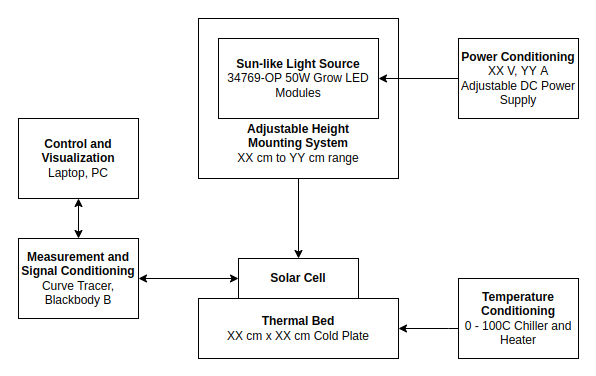
\includegraphics[width=\textwidth]{cell_test_setup.png}
    \caption{Photovoltaic Testing Setup}
    \label{fig:cell_test_setup}
\end{figure}

\begin{figure}[h]
    \centering
    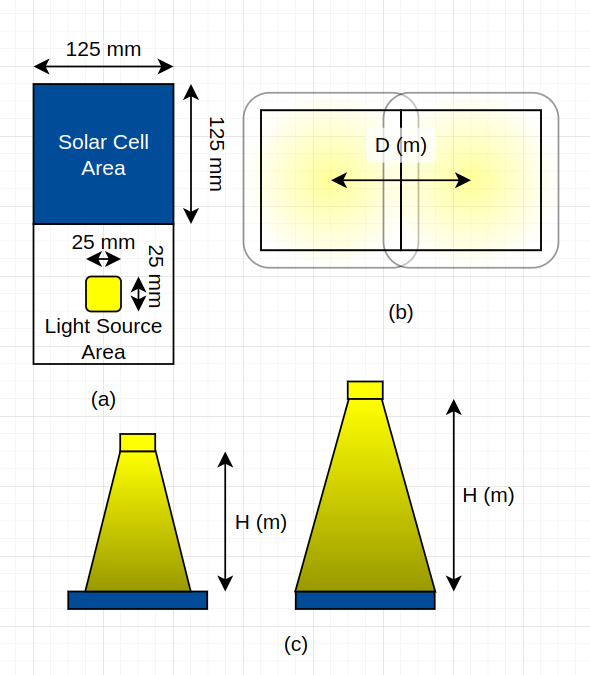
\includegraphics[width=0.6\textwidth]{light_spacing_coherence.png}
    \caption{Grow Light Spacing and Coherence}
    \label{fig:light_spacing_coherence}
\end{figure}

To achieve the last unmet requirement, \textit{the test article shall receive a
measurable and consistent irradiance over the test duration}, the same light
sensor is used to measure the intensity of light over a fixed period of time.
This period of time should be long enough to determine whether the lights have a
warm up time and change in irradiance over the expected experiment duration.
The TSL2591 returns values in counts according to its datasheet, which can be
converted into $\si{watt}/\si{\meter}^2$. However, the normalized responsivity
spectrum of the TSL2591 (\autoref{fig:tsl2591_spectral_responsivity}) is quite
divergent from AM1.5G solar spectrum; this means that the real irradiance will
be off significantly. In order to calibrate the readings from the sensor as a
proxy for the real irradiance experienced by the solar cell, we need to compare
it to either a known source or a reference pyrometer. Another way to interpret
the readings in counts is to convert it into lux; Michael et
al.\cite{michael_et_al} proposes several methodologies for determining and
verifying a $\si{\lux}$ to $\si{\watt}/\si{\meter}^2$ conversion factor. They
also propose an `engineering rule of thumb', that $120 \si{\lux} =
\si{\watt}/\si{\meter}^2$.
\todo[inline]{Add potential note later on about needing teflon to filter in
saturation conditions - can this fixed by adjusting gain/integration time?}
\todo[inline]{Reference Gacusan's, Burgt's thesis regarding designing low-cost
pyranometer using TSL2591 and TSL2591-like sensors}

\begin{figure}[!htbp]
    \centering
    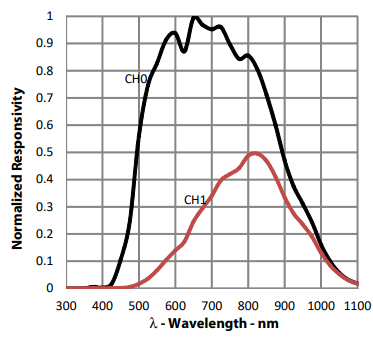
\includegraphics[width=0.5\textwidth]{tsl2591_spectral_responsivity.png}
    \caption{TSL2591 Spectral Responsivity}
    \label{fig:tsl2591_spectral_responsivity}
\end{figure}
\todo[inline]{Add referenceto AMS TSL2591 datasheet. Figure 11.}


\subsection{Experimental Extraction of Cell Parameters}\label{subsec:experimental_extraction_of_cell_parameters}

\todo[inline,caption={}]{
    \begin{itemize}
        \item Present results of each cell line
        \item Compare against smith et al for Gen III how accurate and precise
        the cell distribution is
        \item Review parameters that need to be measured empirically (\ac{RS}, \ac{RSH}, etc)
        \item Discussion on how to measure series and shunt resistance
        empirically (refer to Appendix E)
        \item Discussion on how to measure temperature coefficients empirically
    \end{itemize}
}


\subsection{Statistical Extraction of Cell Parameters}\label{subsec:statistical_extraction_of_cell_parameters}

\todo[inline,caption={}]{
    \begin{itemize}
        \item Review parameters that could be estimated statistically (\ac{alpha}, \ac{beta}, etc)
        \item Discussion on curve fitting techniques
    \end{itemize}
}


\subsection{Modeling Solar Cell Datasets}\label{subsec:modeling_solar_cell_datasets}

\todo[inline,caption={}]{
    \begin{itemize}
        \item Discuss python model for modeling cells, iterative solving (refer
        to Appendix F)
        \item Present initial figures showing expected model output
    \end{itemize}
}


\subsection{Evaluating Solar Cell Models}\label{subsec:evaluating_solar_cell_models}

\newpage
\section{Modeling Solar Modules}\label{sec:modeling_solar_modules}


\newpage
\section{Evaluation of Solar Module Models}\label{sec:evaluation_of_solar_module_models}

\newpage
\section{Modeling Solar Arrays}\label{sec:modeling_solar_arrays}

\newpage
\section{Evaluation of Solar Array Models}\label{sec:evaluation_of_solar_array_models}


\dots
%TODO: conclusion for Chapter 1
\todo{Insert conclusion on chapter topics and results.}
\chapter{Optimizing Photovoltaics}\label{chapter:optimizing_pvs}

% TODO: intro for Chapter 2
\todo{Insert intro paragraph on the focus of this chapter, as well as the a
short discussion of the following sections.}

%TODO: conclusion for Chapter 2
\todo{Insert conclusion on chapter topics and results.}
\chapter{Optimizing Photovoltaic Systems}\label{chapter:optimizing_pv_systems}

% TODO: intro for Chapter 3
\todo{Insert intro paragraph on the focus of this chapter, as well as the a
short discussion of the following sections.}

\todo{Insert sankey diagram from incident light to battery input}

%TODO: conclusion for Chapter 3
\todo{Insert conclusion on chapter topics and results.}


\chapter*{Conclusion}
\addcontentsline{toc}{chapter}{Conclusion}

{
    \hypersetup{linkcolor=black}
    \printbibliography[heading=bibintoc]
    \begin{appendices}
        \chapter{Acronyms and Abbreviations}\label{appendix:acronyms_and_abbreviations}

\begin{acronym}
    \acro{BPS}{battery protection system}
    \acro{CAN}{controller area network}
    \acro{CLI}{command line interface}
    \acro{CLT}{central limit theorem}
    \acro{DC-DC}{direct current to direct current}
    \acro{DRM}{Direct-Reverse Model}
    \acro{EIA}{U.S. Energy Information Administration}
    \acro{GUI}{graphical user interface}
    \acro{GW}{Gigawatts}
    \acro{HW}{hardware}
    \acro{IEA}{International Energy Association}
    \acro{I-V}{current-voltage}
    \acro{LHRs}{Longhorn Racing Solar}
    \acro{MOSFET}{metal-oxide-semiconductor field-effect transistor}
    \acro{MPPT}{maximum power point tracking}
    \acro{MPP}{maximum power point}
    \acro{PCB}{printed circuit board}
    \acro{PPFD}{photosynthetic photon flux density}
    \acro{PV}{photovoltaic}
    \acro{P-V}{power-voltage}
    \acro{SW}{software}
    \acro{STC}{standard test conditions}
    \acro{UN}{United Nations}
    \acro{USB}{universal serial bus}
\end{acronym}
        \chapter{Mathematical Nomenclature}\label{appendix:math_nomenclature}

\begin{acronym}
    \acro{A}[$A$]{area}
    \acro{BS}[$b_S(E)$]{spectral photon flux density}
    \acro{E}[$E$]{energy}
    \acro{EG}[$E_G$]{bandgap}
    \acro{EGREF}[$E_{G,ref}$]{reference bandgap at STC}
    \acro{G}[$G$]{irradiance}
    \acro{GREF}[$G_{ref}$]{reference irradiance at STC}
    \acro{IL}[$I_L$]{load current}
    \acro{ID}[$I_D$]{dark current, or diode current}
    \acro{ID1}[$I_{D1}$]{carrier recombination dark current}
    \acro{ID2}[$I_{D2}$]{surface recombination dark current}
    \acro{IPV}[$I_{PV}$]{photocurrent, or light generated current}
    \acro{ISC}[$I_{SC}$]{short circuit current}
    \acro{ISCREF}[$I_{SC,ref}$]{reference short circuit current at STC}
    \acro{ISH}[$I_{SH}$]{shunt current}
    \acro{I0}[$I_0$]{dark saturation current, or reverse saturation current}
    \acro{I0REF}[$I_{0,ref}$]{reference dark saturation current at STC}
    \acro{KB}[$K_B$]{Boltzmann constant}
    \acro{KE}[$K_E$]{short circuit current constant}
    \acro{N}[$n$]{ideality factor}
    \acro{N1}[$n_1$]{ideality factor of space charge recombination}
    \acro{N2}[$n_2$]{ideality factor of surface recombination}
    \acro{QE}[$QE(E)$]{quantum efficiency}
    \acro{Q}[$q$]{electric charge constant}
    \acro{RL}[$R_L$]{load resistance}
    \acro{RS}[$R_S$]{series resistance}
    \acro{RSREF}[$R_{S,ref}$]{reference series resistance at STC}
    \acro{RSH}[$R_{SH}$]{shunt resistance}
    \acro{RSHREF}[$R_{SH,ref}$]{reference shunt resistance at STC}
    \acro{TC}[$T_C$]{cell temperature}
    \acro{TCREF}[$T_{C,ref}$]{reference cell temperature at STC}
    \acro{VL}[$V_L$]{load voltage}
    \acro{VT}[$V_T$]{thermal voltage}
    \acro{VOC}[$V_{OC}$]{open circuit voltage}
    \acro{VOCREF}[$V_{OC,ref}$]{reference open circuit voltage at STC}
    \acro{ALPHA}[$\alpha$]{short circuit current thermal coefficient}
    \acro{BETA}[$\beta$]{open circuit voltage thermal coefficient}
    \acro{GAMMA}[$\gamma$]{thermal voltage modifier coefficient}
    \acro{ZETA}[$\zeta$]{series resistance thermal coefficient}
    \acro{ETA}[$\eta$]{series resistance irradiance coefficient}
    \acro{KAPPA}[$\kappa$]{shunt resistance thermal coefficient}
    \acro{IOTA}[$\iota$]{shunt resistance irradiance coefficient}
\end{acronym}
        \chapter{Design of a Multi-Channel LED Base Solar Simulator}\label{appendix:solar_simulator}

\begin{itemize}
    \item Measuring light uniformity \href{https://eyehortilux.com/grow-lighting-guide/systems/fixture-uniformity-and-efficiency/}{Fixture Uniformity and How to Measure It}
\end{itemize}

        \chapter{I-V Curve Measurement Using Curve Tracer}\label{appendix:curve_tracer}

        \chapter{Curve Tracer Design}\label{appendix:curve_tracer_design}

        \chapter{Blackbody Design}\label{appendix:blackbody_design}

    \end{appendices}
    \listoftodos[TODOS]
}
\end{document}
